\section*{Project Description}

Testing plays a vital role in modern software development,
contributing crucially to robustness and overall quality---as well as
to overall development costs.
%
It comes in many styles---unit testing, integration testing,
performance testing, stress testing, accessibility testing,
etc.---supported by many sorts of tools, with yet more advanced tools
and techniques continually being developed, studied, and applied.

One such technique, {\em property-based testing} (PBT), has been
enthusiastically taken up by the functional programming research
community since its introduction in the Haskell QuickCheck
library~\cite{ClaessenHughes00}, and is beginning to make
serious inroads beyond academia.
%
PBT is sometimes glossed as ``formal specification without formal
verification'': a developer characterizes the desired behavior of
some piece of code at a high level in the form of executable {\em
  properties}, which are simply Boolean-valued functions. The code is
then validated against these properties by running it over and over
with a large number of automatically generated test cases.
%
PBT tools thus give programmers an efficient way of testing their
code's behavior with a comprehensiveness that is often not
possible with alternative testing methods.

PBT's combination of rich, high-level specifications with easy, mostly
automatic validation has shown itself effective at identifying subtle
bugs in an impressive variety of settings, including telecommunications
software~\cite{arts2006testing}, replicated
file~\cite{hughes2014mysteries} and key-value
stores~\cite{Bornholt2021}, automotive software~\cite{arts2015testing}, and a range
of other real-world systems~\cite{hughes2016experiences}. With support
now available in pretty much every major programming language, PBT has
begun to make significant inroads in the broader software
industry. For example, the developers of the Hypothesis library for
Python estimate that it is used by around half a million
developers~\cite{ZacPersonalCommunication}.

\newcommand{\participant}[1]{{P#1}}
% \newcommand{\participant}[1]{{\bf P#1}}

Given all this momentum, one might wonder if the research community has
already
addressed all of the challenges that could limit PBT's adoption
in the broader software industry.  But it
seems the answer is no.
In an ongoing need-finding study with users of OCaml's QuickCheck testing tool
at Jane Street Capital, we found
consistent enthusiasm for PBT---participants called it it
``obviously valuable'' (Participant \participant{1}),
built their own libraries for it when standard ones were not available in their
development context (\participant{8},
\participant{21}), and suggested that ``everyone'' at the company should use it
(\participant{20}). But we also found
challenging new research questions where advances in technical foundations and
tool design seem necessary to overcome present usability challenges and expand the
potential impact of PBT. \bcp{Last sentence weak.}

Addressing usability challenges in PBT requires insights from both the
programming languages (PL) and
human-computer interaction (HCI) communities.  Chasins et
al.~\cite{chasins_pl_2021} argue that a research methodology
combining PL and HCI hits a ``sweet spot'' where need-finding techniques identify
current pain points and motivate concrete tools that help programmers write
safe, correct programs. We wholeheartedly agree.
Indeed, the team behind this proposal is uniquely positioned to advance the
state of the art in PL and HCI: PI Head recently co-founded
a new HCI group at the University of Pennsylvania and specializes in interactive
programming environments, while PI Pierce has
published widely on PL topics including PBT.

We propose here a comprehensive, interdisciplinary research program on
\emph{usable
property-based testing}, bringing the combined power of PL and HCI to bear to
accelerate PBT's transition into practice.
\begin{itemize}[noitemsep]
\item We will establish a \emph{foundation} for HCI-informed research on PBT,
starting from our ongoing need-finding study. We will confirm
this study's findings and more deeply explore usability of PBT via
two survey studies and an observation study
of PBT users {\em in situ} (\sectionref{sec:foundation}).
  \item We will empower developers to \emph{specify} properties with
  new tools for checking temporal properties over internal program states and
for model-based testing of modularized code (\sectionref{sec:spec}).
  \item We will help developers efficiently define and tune random input
\emph{generators} with novel techniques for generating precondition-satisfying
values, for test input mutation, and for example-based generator
tuning, all building
  on a novel ``reflective'' approach to generation (\sectionref{sec:gen}).
  \item We will support developers in rapidly \emph{validating} testing
  effectiveness with novel interactive tools that help
locate causes of test failures and understand how to improve the
distribution of randomly generated
data to be more representative and comprehensive
(\sectionref{sec:val}).
  \item We will develop materials for PBT \emph{education}
  including an undergraduate computer science curriculum centered around PBT, a
  tool to help students author properties, and a comprehensive review of PBT
  practice to help students and developers identify situations where
  PBT is likely to be most useful (\sectionref{sec:ed}).
\end{itemize}

Success in these efforts will require complementary tools from PL
and HCI research. HCI approaches will be used to concretely define developers' needs,
design the user interface to tools, and evaluate their success. PL approaches
will be used to develop \rewrite{tools such as domain-specific languages and
type-based tools that are powerful and flexible}, and to formally validate these
tools. We conclude the proposal with a concrete outline of our work plan
(\sectionref{sec:plan-of-work}), a discussion of the broader impacts of the
proposed work (\sectionref{sec:broader-impacts}), and a summary of our
prior NSF-supported work.

\subsectionstar{Orientation: Property-Based Testing}
%
\proposecut{To set the stage, we next describe the basics of PBT, with
  the aim of highlighting where research has unique leverage in
  improving PBT tooling, processes, and education}.

Popularized by Haskell's QuickCheck library~\cite{hughes2007quickcheck},
PBT is a form of testing where
executable functions act as partial
specifications of a component under test. For example, a user might
write the following property for an \lstinline{insert}
function for a binary search tree (BST):\footnote{\bcp{No need for a footnote.}The function can be read as
follows:
Assume an arbitrary tree \texttt{t} and an integer
\texttt{x} to insert into that tree. If the original tree
is a BST (``\lstinline{is_bst t}''), then it should remain
a BST after the insertion of \texttt{x} (``\lstinline{is_bst (insert x t)}'').}
\begin{lstlisting}
  prop_insert_correct x t  =  (is_bst t ==> is_bst (insert x t))
\end{lstlisting}
In general, a property is a function that
accepts a generated
test as input and evaluates to \lstinline{True} if the test passes, and
\lstinline{False} otherwise.  This one, ``\verb|prop_insert_correct|'',
checks that an insert operation on a binary search tree preserves the
binary ordering of the tree.
\proposecut{While properties like this one require
only a few lines to express, they can validate unlimited
input-output pairs.}
Given a property, the PBT tool generates a
large number of inputs and
checks that the property yields \lstinline{True} for each one; any input
that causes the property to fail is reported as a {\em counterexample}.

This proposal focuses on {\em random}
generation~\cite{hamlet1994random}, the dominant approach in PBT,
though many of our tools would
also be applicable to alternatives like enumerative test-case
generation~\cite{DBLP:conf/haskell/RuncimanNL08, leancheck} or model
checking\bcp{model checking is not really a generation method}.
The surprising effectiveness of random generation can be attributed to the
``combinatorial'' nature of larger test cases---the fact that bugs can often be
exposed with test inputs that embody a specific combination of features,
independent of whatever other features may be present. For example,
a bug might be triggered by a particular sequence of API calls in a
particular order,
regardless of whether these are
interleaved with other API calls. As a result, testing with large random
inputs often exposes issues much faster than exhaustively enumerating
small inputs.  Techniques like swarm testing~\cite{groce2012swarm} can
further amplify this effect.

To apply PBT, the developer first defines one or more properties that
should be true of the program under test. Then, they write {\em random
  input generators} for the values that the properties take as input
(often these can be automatically generated). Next they check the
properties with generated inputs, using test drivers provided by their
PBT tools. And finally, if counterexamples are discovered, they make
sense of them and determine the source of the bug.  Each of these
steps presents opportunities to improve the user experience of PBT, as
we describe in the next section.

\smallskip

Why go to the trouble of PBT, rather than the more straightforward
example-based testing that is standard across the software industry?
First and foremost because a component can be tested be much more
thoroughly with a property and many automatically generated examples
than with a small number of examples written out by hand.
% \proposecut{As mentioned
% previously, PBT has an impressive track-record uncovering bugs that other
% approaches had failed to
% find~\cite{arts2006testing,hughes2014mysteries,
% Bornholt2021,arts2015testing,hughes2016experiences}.}
But
PBT is more than just thorough---it is also more general than example-based
testing. Wrenn et al.~\cite{wrenn2021using} point out that example-based testing
of programs whose correctness conditions are {\em relational} (e.g.,
topologically sorting a graph, which might correctly
produce any of a number of possible results) is impossible to do
faithfully; a property-based specification is a better choice in
such cases. PBT is also
an obvious choice if formal properties have already been written, as is the case
with tools like QuickChick~\cite{paraskevopoulou_foundational_2015}, which
implements PBT in
the Coq proof assistant.\bcp{I am still uncomfortable with making a
  big deal of this point---it seems weak in the industrial setting.
  (Indeed, even using QuickChick we often have to write properties
  from scratch!)} Finally, the properties required for PBT can also
serve as documentation:
participants in our foundational study (\participant{5}, \participant{21})
talked at length about properties being an ideal way to communicate what a
program is supposed to do.

With all these advantages, it seems clear that PBT belongs on every
software developer's testing toolbelt.  But PBT raises some challenges
as well, as we shall see next.

\subsectionstar{Motivations from a Formative Study of PBT in
Industry\label{sec:motivation}\pagebudget{2}}
%
The work proposed here is motivated by findings from the ongoing
need-finding study we are conducting at Jane Street. The purpose of this
study is to understand how the research community can make PBT more
usable. The study data consists of 30 semistructured interviews
with stakeholders in PBT, including both developers who use PBT and
developers and maintainers of PBT tools.

Jane Street is
an attractive setting for such a study for several reasons.  Most
importantly, PBT is
already well established at Jane Street, so there is a large
population of people with well-informed opinions on its benefits and
challenges. Additionally, Jane Street famously builds almost all of its
software in OCaml, a mostly functional programming language for which
there is a well-engineered PBT tool. This unified
ecosystem ensures that developers have access to mature PBT tools,
experience using them in collaborative settings,
and awareness of language-level abstractions necessary
for advanced usage.
% \footnote{\proposecut{Because our primary need-finding study to-date has
% taken place solely at Jane Street, our follow-up studies in
% \sectionref{sec:foundation} will engage with broader groups of developers using
% PBT to expand and generalize our findings.}\hg{If this is important, it shouldn't be a footnote...}}

As of December 2022, the full complement of 30 interviews has been
completed at Jane Street, and a preliminary round of qualitative
analysis is underway; full-scale analysis will begin in 2023.
Findings from the study will be disseminated in a paper submitted to a
top-tier software engineering conference.  We also carried out a
smaller pilot study among Hypothesis users to prepare for the
full-scale one at Jane Street; this study this was presented at the
2022 HATRA workshop~\cite{goldstein_problems_2022}

\subsectionstar{Framework: Challenges Using PBT} The final result of
the ongoing study will be a deep, qualitative description of how
Jane Street developers use PBT, what they need from it, and how the
research community can
help improve PBT tools. While full analysis of the data remains
to be done, a number themes are already clear in
the interview session notes. These form the backbone of the present proposal.

\newcommand{\proptheme}[1]{{\color{nord-orange} \em #1}}
\newcommand{\gentheme}[1]{{\color{nord-green} \em #1}}
\newcommand{\evaltheme}[1]{{\color{nord-purple} \em #1}}
\newcommand{\edutheme}[1]{{\color{nord-frost4} \em #1}}
A first set of
themes revolves around \proptheme{\normalfont \bf specifications} (i.e.,
properties).
% and the kinds of programs in which they choose to test them.
Since
PBT is often described as a lightweight formal method, one
might imagine that a common challenge would be coming up with the
specifications of desired program behavior. Indeed, in our pilot need-finding
studies with users of Python's Hypothesis library, users indicated just that.
By contrast, Jane Street developers, on the whole, reported
few difficulties coming up with
properties. Rather, most participants described applying PBT in
\proptheme{High-Leverage Scenarios} where properties were already
available or straightforward to invent. For example, participant
9~(\participant{9}) pointed out that PBT was particularly easy to apply when one
has ``a really good abstraction
with a complicated implementation.''
Several participants (\participant{3}, \participant{15},
\participant{20}, \participant{22}), when asked to speculate, guessed
that 80--100\% of Jane Street
developers write programs like this, where properties are easy to find, and
where PBT is relatively easy to apply.  This suggests that an effective way to
improve education and documentation around PBT is to highlight these real-world
applications that seem to be a natural fit for PBT.

It also became clear that there were \proptheme{Opportunities for Better
Leverage} of specifications, where PBT is not easy {\em yet}, but
could be with a little more research effort. For example, many developers in
both our pilot studies (Pilot-\participant{4--6}) and the Jane Street study (\participant{7}) complained
that PBT was difficult when code was poorly abstracted.  We plan to provide
better tool support to address this failure mode.  Furthermore, more than three
quarters of study participants had used a particular approach to PBT commonly
called \proptheme{Model-Based Testing}.  \participant{3}, an author of PBT tools
at Jane Street, considered better automation and tooling around model-based
testing to be one of the most significant ways improve PBT and make it easier to
pick up and use.

Another set of themes concerned the \gentheme{\normalfont \bf generation} of
random inputs for PBT. Developers often spoke
highly of \gentheme{Derived Generators} that can be automatically inferred from
the OCaml type system (\participant{5} called OCaml's tools for this
``[expletive] amazing'' and \participant{30} called them a ``game changer'').
These generators are already quite good, but they could be better: participants
identified deficiencies both small (e.g., API quirks) and large (e.g.,
derived generators
cannot enforce semantic preconditions).

When derived generators
failed, participants fell back to \gentheme{Bespoke Generators}, which
are far more flexible but proportionally more time-consuming to design and work
with. For example, \participant{20} successfully used a bespoke
generator for XML documents to find bugs in their software,
but reported spending ``at least a day'' writing it.
Improving the abstractions available for writing bespoke generators would
greatly improve both the experience of using PBT and its potential for
bug-finding.

If a generated input is determined to be a {\em counterexample} that triggers
property violation, a developer will wish to inspect that counterexample to find
and fix the root cause of the violation. Developers often implemented code for
\gentheme{Shrinking} inputs, or taking counterexamples and discovering smaller,
simpler inputs that trigger the same bug.  \participant{8}
and \participant{21}, who each implemented their own PBT libraries, both
incorporated shrinkers as key components of their libraries. That said,
shrinkers need to be customized to particular kinds of data to be most
effective, and the reality is that they are time-consuming to build; many
developers
(\participant{16}, \participant{20} \participant{21}, \participant{30})
described shrinker implementation as an opaque and difficult process.
Ideally, developers would have tools that make the process of implementing
shrinkers fast and simple.

Further themes from the interview study concerned how developers
\evaltheme{\normalfont \bf validated} their tests.
Developers described their processes for \evaltheme{Evaluating the
Effectiveness} of their tests. Many
desired
better ways to evaluate their generators and properties, including
better feedback on code coverage (\participant{9} and \participant{25}),
incorporation of mutation
testing~\cite{papadakis_mutation_2018}, and understanding the space of generated
inputs (\participant{10}, \participant{16}, \participant{16}). Problematically,
while many developers admitted they would benefit from better tools for
evaluating their tests, many seemed to
\evaltheme{Implicitly Trust the Infrastructure} that they had not thoroughly
analyzed. \participant{14} actually shipped broken code to production because
their generator missed important input examples. We propose advances in tools
for validation that help developers more clearly understand, and improve, the
effectiveness of their tests.

Finally, for PBT tools to be more usable, we need progress in
\edutheme{\normalfont \bf
education}. Developers need to be informed about the \edutheme{High-Leverage
Scenarios} in which PBT should be employed, as we discussed above.
In our pilot studies, we found that developers with less experience with PBT
sometimes struggled to \edutheme{Imagine
Properties}, or understand what properties to test (Pilot-\participant{1},
Pilot-\participant{3},
Pilot-\participant{4}, Pilot-\participant{5}). Developers in both studies
(Pilot-\participant{1}, Pilot-\participant{4}, \participant{3}, and
\participant{11}) reported a dearth of \edutheme{Documentation and Examples} for
learning about PBT. Our final aim in this project is to develop curricula,
documentation, and tools that fill this educational gap.

We discuss plans for work that addresses these themes below, \proptheme{specification
  themes} in \sectionref{sec:spec}, \gentheme{generation themes} in
\sectionref{sec:gen},
  \evaltheme{validation themes} in \sectionref{sec:val}, and \edutheme{education
  themes} in \sectionref{sec:ed}.

\iflater
\amh{Let's foreshadow other findings that
we will publish that are outside of the scope of this proposal, but which might
be motivating to other researchers, including: developers could benefit from
additional automated support for deriving generators from types, effectiveness
budget (i.e., deciding how much time to spend on running PBT tests versus fuzz
tests), integration with unit testing frameworks, and exploring the use of
properties as a source of documentation.}
\bcp{Not sure where is the right place for this discussion (or if
  there will be space)...}
\fi

\SECTION{Foundation}{Understanding Needs and Opportunities%
\pagebudget{1}}{sec:foundation}

% \amh{This section is around double its page budget. One reason is that I am
% probably being too heavy-handed in trying to justify the methodological choices.
% Help me figure out what to prune!}\bcp{Did some pruning! :-)}

The final results from the in-progress user study should paint a clear
picture of the benefits and challenges of PBT in the specific context
of Jane Street and other organizations with similar characteristics.  But to
fully understand the potential impact of PBT across the software
industry---and the factors that may limit its adoption---we need to
cast a wider net.
%
In this section, we describe three planned studies, drawing on mixed
methods in the service of producing a comprehensive and actionable
agenda for future research, in this research project and beyond---two
written surveys, one to assess the generality of these needs and obstacles
and one to identify potential for adoption of PBT tools
(\sectionref{sec:survey}), and an observation study to understand
particular tasks involved in PBT to guide the design of new algorithms
and interactive tools (\sectionref{sec:observations}).

\SUBSECTION{Generalizing the Jane Street Findings}{sec:survey}{2}{3}{Other}
%
Our ongoing Jane Street study has already revealed a number of
opportunities to improve tools for property-based testing. To identify
others and to better understand which of these opportunities are most
important for the research community to explore, we will conduct two
surveys with broader samples of developers. These surveys aim to
(1) determine which obstacles observed in the interview study
represent widely experienced pain points with PBT tools and
(2) characterize the potential benefits of better tools to the
software industry as a whole.

\emph{Validation survey}. The main survey we plan to conduct aims to check that
the things we learned from Jane Street generalize more broadly.
Our interview study has revealed
a number of issues with existing PBT tools, but it is not clear
how broadly these issues are experienced by developers, or
their relative severity. To find out, we will
ask developers which of the issues we have identified are
ones they have experienced, and the severity of those issues
in their experience. Respondents will also be asked to report on
other issues they encountered in their use of PBT tools.
To provide
clear usage scenarios to guide future work, respondents will
be asked to write brief anecdotes elaborating on the
most severe issues they had.

Respondents will
be recruited broadly, from three sources: (1)
users of Hypothesis, a widely used Python-based PBT
framework; (2) Jane Street, reaching
a broader set of developers than we were able to interview; (3)
through word of mouth, via announcements on the PIs' Twitter and Mastodon
accounts, various mailing lists, and discussion boards for conferences like
``Yow!'' where we have been invited to speak~\cite{noauthor_when_nodate}.
% Types and types-announce mailing lists. They are mailing
% lists for the types programming. We will distribute announcements among
% attendees of conferences like ICFP or ``Yow!'' whom have
% a cumulative thousands of programmers with functional
% programming experience.

\emph{Impact survey}. Another more speculative survey we hope to conduct asks
how broadly PBT may eventually be able to reach.  To get a sense of this, we
survey ``proximal'' users of PBT---that is, developers who do not use PBT
currently, but who experience use cases where PBT methods would be particularly
useful.  Particular attention will be given to those whose work requires the
writing of validation code and public APIs with some definition of types. We
will recruit a broad sample of participants across development contexts
(professional, open source, educational) by working with our industry contacts
and by recruiting over social media. Admittedly, this survey seems more
difficult to ``get right,'' and the design will evolve over time as we gain a
better understanding of the situations where PBT is most effective
(see \sectionref{sec:whento}), but if done right this could provide invaluable
feedback to PBT researchers about how far their work could reach.

\SUBSECTION{Observing PBT in Practice}{sec:observations}{3}{4}{Other}
%
Anecdotes related in interviews do not generally, in and of
themselves, provide enough information to inform the design of
effective tools---they beg questions like: (1) How much time
are participants willing to devote to
a task like creating a generator or debugging a counterexample when in the
middle of a programming task? (2) How much space is available on a developer's
screen (amidst other tools like code editors and terminals) for
new
tools? (3) What are developers' current strategies for solving the
problems they describe
(e.g., what representations of generated data currently seem most helpful
for programmers trying to understand the distributions of data generated by a
generator)? As a basis for designing tools with a substantial novel interface
component (see \sectionref{sec:val}), we will observe developers
undertaking the respective PBT tasks we
aim to support, on the order of a small handful of developers (i.e., 2--10
observation sessions). These observations will allow us to evolve
singular anecdotes from the interviews into a more comprehensive picture of
what kinds of designs will be viable for helping programmers.


\SECTION{Specification}{Widening the On-Ramp\pagebudget{2}}{sec:spec}
The projects in this section address the challenges related to
\proptheme{specification} discussed in the motivation section. One major finding
of the study is that widening the on-ramp to PBT requires making developers
aware of high-leverage use-cases for PBT. We discuss our plans to teach developers
about high-leverage scenarios in \sectionref{sec:whento}; in this section, we
discuss opportunities to expand and improve the space of scenarios where PBT
shines.  In we improve PBT's applicability to poorly abstracted code
(\sectionref{sec:outpurprop}), and we describe tools that automate
automatically in a specific high-leverage scenario: model-based testing
(\sectionref{sec:automating}).  Together, these projects will greatly improve
the on-ramp to PBT and clarify its place in the software industry.

\SUBSECTION{Properties Over Logs}{sec:outpurprop}{1}{2}{Harry}
As discussed in the motivation section above, a common problem
raised by Jane Street
developers (and even more loudly in our earlier pilot
study~\cite{ref:goldstein2022some}) was that code may sometimes not be
abstracted in a way that is amenable to testing. Indeed, any kind of
testing of software units---with PBT techniques or otherwise---requires
``units'' to test!  But PBT is
especially sensitive to issues like poorly encapsulated global state, which may
impact the repeatability of testing, and leaky or confusing
abstraction boundaries, which make it difficult to cleanly state
properties or specifications.

For example, one developer (\participant{7}) described their experience testing a
system (we'll call it \lstinline{Inner}) with messy abstraction
boundaries. In this case, \lstinline{Inner} was hard to test because it was
primarily used as a sub-component of a larger system \lstinline{Outer};
\lstinline{Outer} would take in simple data, and then at some point pass a
large, complex data structure to \lstinline{Inner}, which would do some work and
hand results back to \lstinline{Outer}. PBT of \lstinline{Inner} was therefore
hard, because generating valid examples of the large data structure that
\lstinline{Inner} takes as input required deep knowledge of the internals and
types of \lstinline{Outer} that the developers of \lstinline{Inner} did not have
access to, and because the interface was too complex to write straightforward
properties about.

We propose a novel approach to testing systems like \lstinline{Inner} that are
difficult to write properties about because they cannot be fully extracted from
a larger system.
At its core, this approach tests
\lstinline{Inner} through \lstinline{Outer} by
writing properties over intermediate values in \lstinline{Inner}. Properties like
\begin{lstlisting}
  sublist_of processed (next (processed))      (* 1. Processing is monotonic. *)
  msg.length < 100 ==> never (overflow = true) (* 2. Capacity at least 100 bytes. *)
  eventually (processed.length = msg.length)   (* 3. The whole message is processed. *)
\end{lstlisting}
which demonstrate that internal variables like \lstinline{processed},
\lstinline{msg}, and \lstinline{overflow} evolve correctly over time, let the
developer talk about the behavior of \lstinline{Innner} without talking about
its external-facing API.
These properties could theoretically be tested without ever running
\lstinline{Inner} on its own: we can generate inputs to \lstinline{Outer}, have
\lstinline{Outer} drive \lstinline{Inner}, and simply monitor the variable
values to check the desired properties.

The tricky part comes with how to actually implement this testing. One might
hope to do it through debug assertions, but that quickly becomes untenable.
Checking the property (1) with debug assertions would require noisy code to
saves the previous value every time \lstinline{processed} is updated, and the
programmer would need to use macros or some other kind of meta-programming to
remove that code when building in release mode. Even worse, there may be no way
to check properties (2) or (3) at all. Doing so would require making an
assertion at the ``end'' of the computation, which may not actually be possible
if \lstinline{Outer} is driving \lstinline{Inner} from the outside.

Instead, we propose a framework for writing properties over {\em logged values}
that can capture the interesting relationships between past and future variable
values that the above properties demand.  Concretely, we will insert lightweight
logging annotations and provide a language for writing properties over those
logs. In order to express concepts like \lstinline{next}, \lstinline{never}, and
\lstinline{eventually} the property language will need some logical connectives
that are not standard in PBT.  In particular, we need a temporal logic like {\em
linear temporal logic} (LTL) so that properties can capture a notion of time.

Using LTL with PBT is not unheard of---Quickstrom testing
framework~\cite{oconnor_quickstrom_2022} has already shown that LTL properties
can be used for specifying and testing graphical user interfaces---but LTL
properties at this level of generality have not yet been attempted. We plan to
compile the user's LTL formulae to properties over traces that respect the
structure of the log and ignore updates to irrelevant variables. Then, the
developer can provide inputs to some system containing the sub-system under
test, and the test harness will apply the trace properties in real time. In this
way, the user can get feedback about the invariants that should hold of the
intermediate values of their programs, making PBT available in a huge range of
programs where it was previously too difficult to apply.

\SUBSECTION{Models for Modules}{sec:automating}{2}{3}{Harry}
One finding that has surprised us from the Jane Street study is that
it is {very} common for developers to build (or already to have) a
{\em model
implementation} of the code they are testing and check that the two versions of
the same code produce the same results.  This is a well-documented approach to
PBT~\cite{hughes_experiences_2016}, but it is not supported as well as it could
be by existing tooling.
%
With this in mind, we propose comprehensive tooling to automate
model-based testing for a large class of ML-style software
{\em modules}~\cite{macqueen_modules_1984}.

\begin{figure}[t]
  \begin{minipage}{.45\textwidth}
\begin{lstlisting}
module StringFns : sig
  val reverse : string -> string
  val drop_n  : int -> string -> string
  val split   : string -> string * string
\end{lstlisting}
  \end{minipage}
  \qquad\qquad
  \begin{minipage}{.45\textwidth}
\begin{lstlisting}
module Set : sig
  type 'a t     val empty : 'a t
  val mem   : 'a t -> 'a -> bool
  val add   : 'a t -> 'a -> 'a t
\end{lstlisting}
  \end{minipage}
  \vspace{-4mm}
  \caption{Some module interfaces we would like to test
    automatically.}\label{fig:sigs}
\end{figure}

Model-based testing is trivial in the simplest case (comparing two pure
functions), but if the code under test is a {\em collection} of functions,
organized into a module, things get more interesting. Testing even a simple
module requires a complex orchestration of calls to the different functions in
the module's signature. For example, testing \lstinline{StringFn} (in
Figure~\ref{fig:sigs}) correctly requires wiring up the functions in the
signature to satisfy their types: \lstinline{drop_n} needs a randomly generated
integer to know how much to drop, \lstinline{split} produces a pair of strings
that can each be arguments to future function calls, etc. We will build on prior
work~\cite{hughes_experiences_2016} to correctly generate well-typed sequences of function
calls that can be used to compare module implementations.

Testing modules gets even hairier when they contain {\em abstract types}, as is
the case with \lstinline{Set}. Now, some of the types in the signature cannot be
generated on their own, so they must be built up from scratch (in this case by
calling \lstinline{create} and \lstinline{add}). The \lstinline{Set} module is
also {\em polymorphic}, so a type must be chosen for \lstinline{'a} before
testing. (There is significant work on this
problem~\cite{hou_favonia_logarithm_2022}, but it is not solved in general.)
To solve these problems, we will take a theoretical approach, breaking down
modules theoretically and developing automation heuristics from first
principles. This process will necessarily involve carving out some subset of
modules where automation is not possible, but highlighting that subset will
provide useful context for future work in PBT usability.

% \proposecut{%
% Finally, so far we have only talked about comparing implementations of the same
% module signature, but what about implementations of {\em related} signatures? In
% theory, it should be possible to automate test harnesses when two modules share
% some subset of behaviors, or when the concrete types that they operate on are
% related in some known way. We will work with users to understand the
% important use-cases.
% }\amh{Can this be removed? The paragraphs above already feel like the most central parts
% of this idea, punchy, and interesting.}

\SECTION{Generation}{Better Tools for Random Inputs\pagebudget{3}}{sec:gen}
%
The Jane Street study highlighted several \gentheme{generation themes}.
Generators were regularly cited as one of the most challenging parts of the PBT
process---the existing tools for random generation are varied and powerful, but
they are not very usable.  In this section, we discuss {\em reflective
generators}, an abstraction for random generation, currently under development,
that exposes levers for
automation that enable a host of new approaches to generator
tooling (\sectionref{sec:reflective}). Reflective generators enable new
approaches to shrinking (\sectionref{sec:shrinking}) and fuzzing
(\sectionref{sec:fuzzing}) that reduce developer effort and improve testing
effectiveness.

\subsectionstar{Context: Random Generation is Hard}
As discussed in the Orientation section above, PBT relies heavily on {\em random data
generators}. The inputs produced by the generator exercise the developer's
properties and give confidence that they hold---provided the inputs are
interesting enough.
%
However,
many properties that developers want to test have {\em preconditions}
(or {\em validity conditions} or {\em input constraints}) that
restrict the set of inputs that should be used for testing. This comes up often
when testing data structures with invariants that must hold in order to apply
the operations under test. Testing such properties can be problematic, because
many preconditions are difficult to satisfy randomly; if the developer is not
careful they may waste most of their testing time generating and
discarding invalid inputs.
%
Worse, even among valid inputs, not all are equally realistic. Often generated inputs
feel fabricated, since they are not constructed with prior knowledge of the
kinds of inputs that the program is likely to see.
%
Worse yet, even with validity and realism accounted for, there are
other ways for generators to under-perform---for example, by
generating many overly similar inputs while ignoring large parts of
the input space.

% The PBT literature partially addresses these concerns, with solutions solving
% one problem at the expense of another and trading off between programmer effort
% and generator power.

Existing approaches to these issues
fall on a spectrum from automatic to manual. The automatic approaches use
proxies for validity and general ``interestingness'' of inputs: some, like {\em
fuzzers}~\cite{afl-readme}, optimize readily available metrics like code
coverage, others ask users to provide metrics~\cite{loscher2017targetedpbt}, and
naturally some use machine learning to infer proxies for
validity~\cite{godefroid2017learn, DBLP:conf/icse/ReddyLPS20}. These approaches
are easy to apply and can obtain good distribution coverage, but they are rarely
sufficient for testing properties with complex preconditions. Slightly more
manual approaches are based on declarative representations of validity
conditions: for preconditions that are primarily structural, {\em grammar-based
fuzzing} provides a compelling solution~\cite{godefroid2008grammar,
holler2012fuzzing, veggalam2016ifuzzer, wang2019superion,
srivastava2021gramatron}, and for more complex, semantic preconditions, some
have proposed using SMT-solvers~\cite{dewey2017automated, LuckPOPL,
steinhofel2022input} to automatically seek out valid inputs. These tools are
much better at satisfying up to moderately-complex properties, but some are
still out of reach. The semi-automatic
category also includes tools for {\em example-based tuning}, a process that
improves realism of inputs by mimicking user-provided
examples~\cite{soremekun2020inputs}; the existing tools successfully generate
more realistic inputs, but are again limited in the preconditions they can
satisfy.

\subsectionstar{Context: Monadic and Free Generators}
\iflater\hg{Not sure I love this transition... I liked it better when this sentence was above}\fi
The most manual, but also the most flexible, solutions use hand-written
generators, written in a convenient domain-specific language (DSL).
In  Haskell, where PBT was
first popularized, many such DSLs are implemented using {\em
monads\/}~\cite{moggi1991notions}, an elegant design pattern for
expressing effectful (in this case, random and stateful) computations
in a pure, stateless underlying
language. While monadic DSLs are not actually necessary to express generators in
non-pure languages, some libraries (e.g., in OCaml) still use monadic
abstractions to build their generator DSLs.

Monadic generators can implement random data producers of arbitrary complexity
(e.g., it is possible to write a monadic generator for Haskell
programs~\cite{palka_testing_2011}), so they are often more expressive than
other representations like grammar-based generators.  Yet monadic generators are
syntactically constrained in a way that isolates the probabilistic code and
prevents usage errors (like passing the wrong random seed around). As we will
see, the constrained nature of monadic generators also makes them the perfect
candidates for sophisticated manipulations and interesting generalizations.

In order to improve monadic generation along the dimensions listed
above, it helps to re-frame generators as {\em parsers of randomness}. A generator
operates by making a series of random choices, but we can equivalently think of
it as being provided some random sequence of choices and then simply following
those choices to produce a value. This perspective has been used in a few
implementations of PBT
systems~\cite{maciver2019hypothesis, dolan2017testing}; we made it
formal in our paper, {\em Parsing Randomness}~\cite{goldstein2022parsing}.
%
This paper introduced {\em free generators}, which generalize the standard
monadic generator abstraction, demonstrate a formal link between parsing and
random generation, and enable new algorithms for generation that improve
generation modulo validity constraints. Free generators are written the same
way as standard monadic generators, but in reality they are more like
generator ``plans'' or syntax trees.%
\footnote{For experts: Free generators are implemented using {\em freer
monads}~\cite{kiselyov2015freer}, which have been used to great effect in recent
years to capture the structure of effectful computations
(cf.~ITrees~\cite{old:xia2019interaction}). Freer monads represent
monadic computations syntactically by reifying the monad operations
(\lstinline{return} and \lstinline{>>=}) as data constructors. Critically, this
is all implemented within the language (no macros or AST
manipulation). See \cite{goldstein2022parsing} for more details on the
free generator representation.}
In {\em Parsing Randomness} we proved that any free
generator can be interpreted
either as a standard monadic generator or as a source of
random choice strings with a parser over those strings; this formalizes the
relationship between generators and parsers.

\SUBSECTION{Reflective Generators}{sec:reflective}{1}{2}{Harry}
Building on the free generator work described above, we have begun to look at
yet more powerful generalizations of the standard monadic approach to random
generation. The most promising of these concerns monadic generators that
can be run {\em backward}.
%
If a generator parses a sequence of choices into a value, then running the
generator backward should take a value and produce a sequence of choices that
would produce that value. With this in mind, we have begun working on {\em reflective
generators}, an extension of monadic generators that can be run backward to
``reflect'' on the choices that they made when producing an input. The machinery
that makes reflective generators work is quite complex,%
\footnote{Reflective generators are both monads and {\em
    partial profunctors},
implementing bidirectional programming in the style of Xia et
al.~\cite{xia2019composing}. This approach to bidirectional programming is
related to lenses~\cite{foster2009bidirectional}, but it hides much of the
complexity of bidirectional program composition in the bind operation of the
monad. The result is an elegant programming experience where both directions of
the computation can be written at once, in a type-safe way.}
but, like free generators, their syntax is still close to that of normal
monadic generators.

Note that the backward direction of reflective generators is different from
remembering the choices the generator makes as it goes (which is already
commonly done~\cite{maciver2019hypothesis,hatfield-dodds_hypofuzz_nodate}). For
one, the generator can reflect on choices for inputs it did not produce itself,
and for another the choices can be given different structures (bit strings,
higher-level choice strings, choice trees, etc.) depending on the needs of the
caller.

The bidirectional nature of reflective generators makes them useful
for more than just generation!  We have begun exploring two other
applications...

{\em Validity-Preserving Mutation.}
Many automated testing algorithms
(especially fuzzing algorithms~\cite{afl-readme}) {\em mutate} values
so as to explore
the behavior of the program in a space ``around'' those
values. Mutation can be
difficult in PBT scenarios, where values are subject to complex validity
constraints, since mutation often produces invalid values. Reflective
generators can help here: We can (1) reflect on the choices that lead
to a particular
value, (2) mutate those choices, and (3) re-run the generator with the new
choices {\em while correcting any choices that
would lead to an invalid value.} Figure~\ref{fig:mutation} shows the way this
algorithm is able to mutate a binary search tree, while maintaining validity,
using no BST-specific code beyond the reflective generator itself.
\begin{figure}[h]
  \centering
  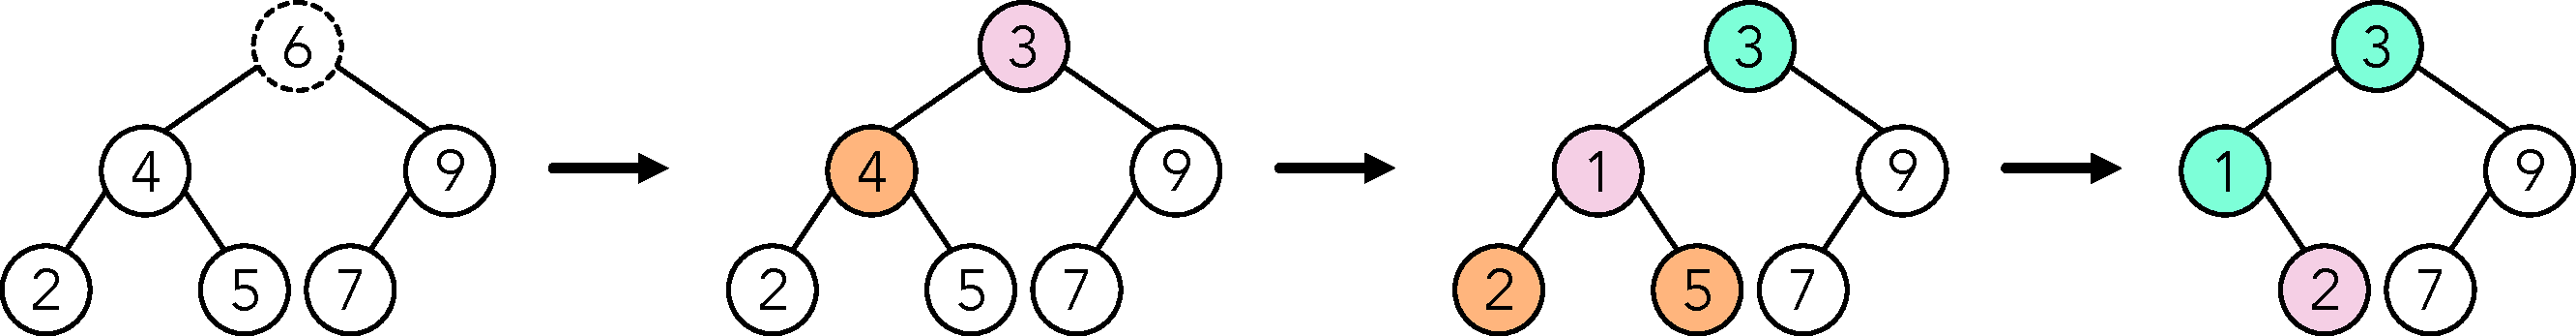
\includegraphics[width=.6\textwidth]{assets/mutate-diagram.pdf}
  \vspace{-2mm}
  \caption{Validity-preserving mutation of a binary search tree, maintaining the
  BST invariant.}\label{fig:mutation}
\end{figure}

{\em Example-Based Tuning.} Earlier we pointed out that good generators
produce ``realistic'' inputs; one way to ensure this is to tune the generator so
it produces values that are similar to some user-supplied values deemed
realistic. Existing tools make good use of this example-based approach to
tuning~\cite{soremekun2020inputs}, but they do not work with generators as
powerful as monadic generators. We implement a similar algorithm using
reflective generators: we can (1) again, reflect on the choices that lead to a
set of realistic values, and (2) run the generator with {\em new choice weights}
informed by the choices that we saw.

Both of these applications have the potential to significantly improve
testing effectiveness---example-based tuning helps users generate more
realistic inputs, while validity-preserving mutation enables more
automated approaches to improving generator distributions---and we get
{\em both} by upgrading our generators to reflective ones. We
demonstrate additional use cases for reflective generators in the
following sections.

\smallskip

{\bf Status.}\bcp{After some agonizing, I decided to try moving it
  here.  WDYT?}  We began thinking about the design of reflective
generators in the context of an earlier NSF project (described in
\sectionref{sec:prior}), built a prototype implementation, and drafted
a preliminary progress report~\cite{Frohlich2022}.  Many details of
both theory and implementation remain to be ironed out; in particular,
while exploratory empirical evaluations look promising, more thorough
experimentation will be required.


\SUBSECTION{Reflective Shrinkers}{sec:shrinking}{2}{2}{Harry}
%
Reflective generators' ability to run backward means that they can be used as
part of any algorithm that needs to understand the structure of generated
inputs.  We therefore propose using them to implement validity-preserving {\em
shrinking} of values to find smaller counterexamples and speed up debugging
without any more effort from the user. On its face, this feels similar to
validity-preserving mutation: Can we reflect on choices, shrink the choices, and
then re-run the generator with the smaller choices? Likely yes! But there are
complications.

Shrinkers need to be more careful than mutators to keep shrunk values faithful
to the original. When mutating, it is often fine if the mutated value is
accidentally quite different from the original value, since the mutator is
trying many values and any that catch a bug are equally good. But a rogue
shrinker runs the risk of confusing the developer much more than they already
were. For example, if a reflective shrinker accidentally creates a visually larger
value, for example, because the relationship between choice sequence length and
output value size is not monotonic, the shrinker might actually make it more
difficult to find a bug. Additionally, if a reflective shrinker's shrunk choices
produce a values that are very different from the original, they may fail to
shrink at all, instead just stepping to values that are no longer
counterexamples and concluding that the original value is a local minimum.

In order to establish reflective shrinkers as a once-and-for-all solution to
validity preserving shrinking, we plan to formalize and prove the above
properties. Specifically, we want to show that, for some class of reflective
generators, the associated reflective shrinkers (1) never produce larger values
with fewer choices and (2) always produce shrunk values that are ``close'' to
the original. Formalizing sub-classes of well-behaved reflective generators and
notions of ``shrinker closeness'' will also give valuable insights into other
applications of reflective generators and shrinkers.

We mentioned in the motivation section that participants in the study thought of
shrinking as magical, but currently the abstraction is too leaky for them to
be comfortable ignoring it.  Our hope is that eventually, having a reflective
generator on hand will mean that shrinking, even in the face of complex
preconditions, is {\em actually magic}, requiring no developer intervention and
making counterexamples far easier to understand.

\SUBSECTION{Reflective Fuzzers}{sec:fuzzing}{2}{3}{Harry}
{\em Fuzzers} like AFL~\cite{afl-readme} use principles that are similar to the
ones behind PBT: they leverage randomized testing to quickly exercise as many
program behaviors as possible. Fuzzers are compelling because they are
inherently easy to use. The developer need only point the fuzzer at a binary and
wait for it to find bugs. But without help, fuzzers are not very good at finding
bugs in programs with complex preconditions.

There are a rew existing projects that try to get the best of both worlds by
combining PBT and fuzzing.
For example, the FuzzChick library in Coq~\cite{OLDlampropoulos19fuzzchick}
uses code coverage as guidance for PBT and the HypoFuzz library uses a
similar approach in Python~\cite{hatfield-dodds_hypofuzz_nodate}. These projects
are demonstrably powerful, but neither benefits from the years of expertise
poured into industrial-strength fuzzers; Crowbar
does~\cite{dolan2017testing}. Crowbar uses
AFL~\cite{afl-readme}, one of the best-established
fuzzers, to generate random bit-strings that are later parsed into program
inputs. Crowbar does require more user effort than standard fuzzing techniques,
but the coverage-guidance means that careful tuning is often not required to get
good testing performance.

We like the model of Crowbar a lot, but think it does not quite go far enough;
we intend to replicate a version of Crowbar built on reflective generators that
is even more powerful.
We start with a classic fuzzing setup, attempting to make the system under test
crash by passing it a variety of semi-random inputs. Normally, the fuzzer is
working against the parser, in the sense that the parser's job is to reject
invalid inputs and the fuzzer's job is to ``get past the parser.'' Crowbar's
generators avoid this adversarial relationship and subsume grammar-based
generation with a powerful generator that is powerful enough to satisfy the
parser by construction; ours will as well, but with reflective generators.

Why use a reflective generator? First, we should clarify why any kind of monadic
generator is preferable to grammar-based options. Monadic generators can
straightforwardly generate context-free structures, and they can often do so
automatically with the help of type information~\cite{mista2019deriving}. If
this is all that the precondition requires, then there is no harm in using a
monadic generator, rather than a grammar-based one. But the beauty of a monadic
generator is that it can be made far more powerful, incrementally, as the
developer's testing needs change. The developer can start off thinking that they
need only consider the structure of their inputs, but they can later add more
semantic guarantees if they determine that their testing is ineffective.

Focusing on reflective generators specifically, one compelling benefit is that
their backward interpretation can be used to help seed the fuzzer.  Most fuzzers
ask for a number of {\em seeds}, input examples that the fuzzer can start from,
in order to ensure that the fuzzer does not spend ages exploring
inputs that have no hope of working out. Normally these seeds are easy enough
for the user to write down, since they are simply program inputs, but now that
we are asking the fuzzer to generate sequences of choices it becomes much more
error-prone (and tedious) to produce seeds by hand.  This is one great use for a
backward interpretation. The user can write down their seeds---either as values
in the program, or as text that can be parsed by the program's parser---and then
the reflective generator can reflect on the choices that produce those seeds.

The reflective generator also provides validity-preserving mutation. Guided by
heuristics, the system can opt to supplement the fuzzer's mutation schedule with
mutations that are obtained by the reflective generator's validity-preserving
mutation (which is more targeted than the mutators provided by the fuzzer). We
expect this to have a significant impact on performance, especially in contexts
where preconditions are relatively sparse and therefore hard for AFL to mutate
correctly.

Our ultimate goal is a unification of PBT and fuzzing tooling that combines the
powerful automation potential of reflective generators with the usability of
fuzzers. Testers will be able to test properties with complex preconditions
without giving up the power and simplicity of coverage-guided generation.

% \SUBSECTION{Benchmarking}{sec:benchmarking}{1}{3}{Other}
% \iflater\todo{Make sure this feels different from Leo's CAREER}\fi
% \bcp{Maybe we should just cut it!}
% %
% The many papers in the PBT literature demonstrate effectiveness with case
% studies, showing that certain bugs in certain systems are caught more quickly
% with one too over another. For theoretical advances, this is often sufficient
% to demonstrate that the paper is worth publishing, but this kind of evaluation
% can be hard to interpret from the perspective of a would-be user. With all of
% the new approaches to generation that we are proposing in this document, and
% considering our goals around usability, we want to do better.

% We will to develop and popularize a robust empirical evaluation framework for
% generators and other PBT techniques. Our first contribution will be an
% infrastructure for easily and extensibly running experiments.  By ``easily,'' we
% mean that we will take on the burden of collecting data and analyzing the
% results, exposing to the user library functions for their particular
% instantiations as needed. We will evaluate a given tool based on (1) the degree
% to which it is able to achieve high code coverage quickly, and (2) the speed
% with which it finds bugs that have been pre-seeded in example programs. By
% ``extensibly,'' we mean that in addition to the two languages (Haskell and
% OCaml/Coq), multiple frameworks (QuickCheck, SmallCheck, QuickChick, etc.), and
% numerous workloads that we plan to support on release, we will design the
% infrastructure so that users can easily add new things along each dimension.

% Our second contribution will codify a library of case-studies and examples as
% {\em benchmarks for PBT}. Similar suites of benchmarks already exist in the
% fuzzing literature~\cite{hazimeh_magma_2021}, but those benchmarks are not
% organized around the particular challenges that PBT tools face. In particular,
% few of the benchmarks deal with the kinds of complex preconditions that PBT
% tools are built to handle. We want to establish a set of challenging tasks that
% can serve as a north star for future improvements to PBT generators and
% bug-finding strategies (including our own!).

% Designs for this project are currently being discussed with Leonidas
% Lampropoulos and his group at the University of Maryland. PI Pierce has a long
% history of successful projects with Prof.
% Lampropoulos~\cite[etc.]{LuckPOPL,goldstein2021dojudgeatest,lampropoulos_coverage_2019,Lampropoulos&18,OLDlampropoulos19fuzzchick}.
% \iflater
% \hg{Is this everything? Probably not...}
% \fi

\SECTION{Validation}{Understanding Testing Effectiveness%
 \pagebudget{3}}{sec:val}

Another major challenge in maximizing PBT's usability helping developers
\evaltheme{validate} that their testing is effective. In this section, we
describe a sequence of research efforts to design and evaluate usable developer
tooling for PBT. These projects will contribute new paradigms for tools that
help developers assess whether their generators are generating sufficient and
appropriate inputs (\sectionref{sec:evaluating_distributions}) and whether those
inputs sufficiently exercise their code (\sectionref{sec:tuning}), migrate
failing property-based tests into regression tests (\sectionref{sec:counter}),
and understand testing-provoked failures involving complex inputs
(\sectionref{sec:failures}). These projects will be pursued using HCI
methodology, integrating these tools into contemporary interactive development
environments. PI Head will guide tool development efforts leveraging his
experience designing, developing, evaluating, and deploying programming
environments and tools~\cite{ref:head2015tutorons,ref:suzuki2017tracediff,ref:head2017writing,ref:head2018when,ref:head2018interactive,ref:head2019managing,ref:head2020composing}.

\SUBSECTION{Evaluating Data Distributions}{sec:evaluating_distributions}{2}{3}{Other}
%
In comparison to testing techniques like unit testing, PBT focuses on testing
distributions of inputs, rather than individual inputs. The success
PBT depends on a developer's ability to create a distribution
of input data that is sufficiently realistic and comprehensive. We plan
to develop much-needed tooling for
understanding distributions of input data and easily changing them.
% This was a pain point of participants in our study, many of whom
% did not know the kinds of input their generators were producing.

We draw inspiration from related work in HCI that has sought to better expose
the shape of input data distributions including
machine learning datasets
(e.g.,~\cite{ref:hohman2019gamut} and
~\cite{ref:hohman2020understanding}) and sequences of program values
(e.g.,~\cite{ref:kang2017omnicode}).
PBT poses a unique challenge because values produced by generators are
programmatically generated and
can be of unbounded structural
complexity (e.g., lists, trees, and other algebraic data types).
Consider an
example from a participant in our formative study, who wanted to generate
realistic logs of input data, where each log entry included at least a timestamp
and an event type. Such values are not trivially plotted in conventional
visualizations, and it would be prohibitive to review individual examples if the
logs are sufficiently long. Ideally, a developer would be able to answer
questions like: Are the generated log inputs long enough? Are the even sequences
realistic? This setting requires new kinds of views of data, and tight
developer support for easily defining meaningful views of the data.

\begin{wrapfigure}{r}{0.58\textwidth}
  \centering
  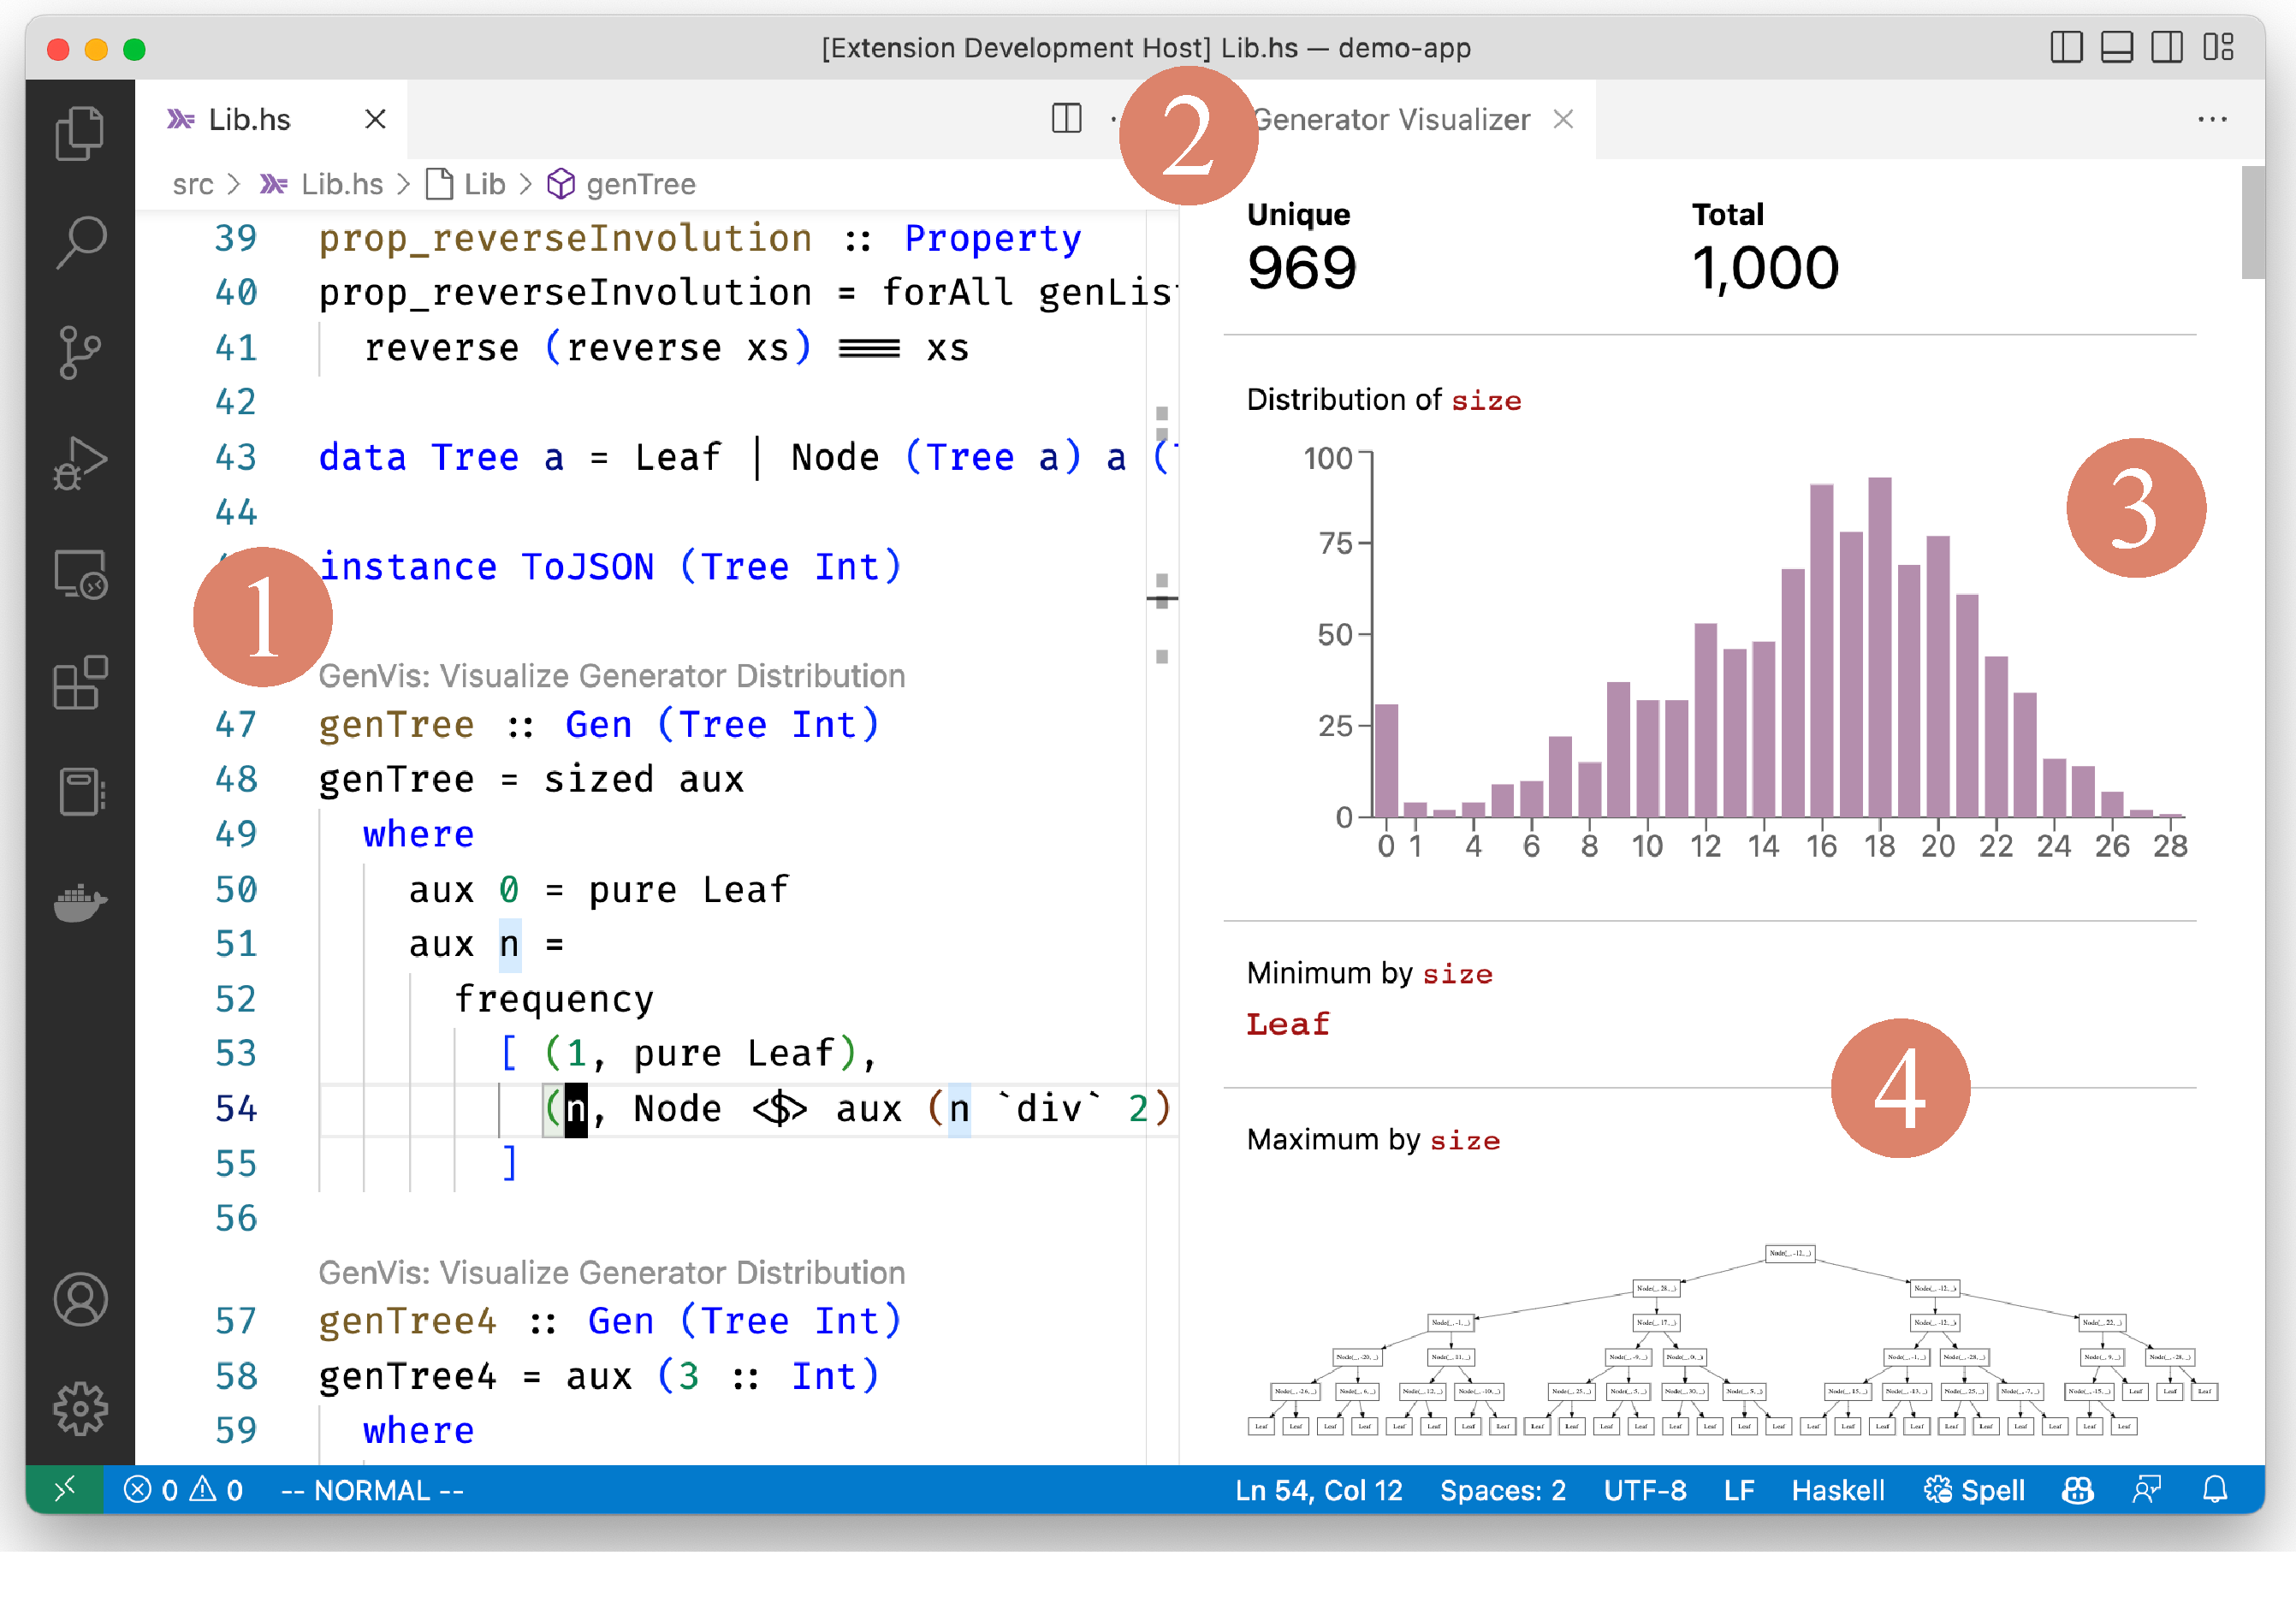
\includegraphics[width=0.58\textwidth]{assets/gen-vis.pdf}
  \caption{An envisioned tool for evaluating data distributions.}\label{fig:gen-vis}
\end{wrapfigure}

To this end, we will design new interactive tools that provide rapid,
informative views of input data distributions. The tools will address the
challenges of visualizing generator distributions using a novel combination of
tailored, tried-and-true features for interactive programming environments.

First, the tool will support live, realtime displays of generated values.
Because PBT takes some time to run, our first goal is to provide
instant, live~\cite{ref:tanimoto1990viva} feedback on the generators. Building
in the tradition of other live functional programming environments
(e.g.,~\cite{tool:lighttable,ref:omar2019live}), our environment will provide
live feedback on the many inputs associated with the code, rather than a single
input. As the test runs, our tool will sample inputs output by the generator and
pipe them into data displays (Figure~\ref{fig:gen-vis}). These data displays
will first and foremost show aggregate data views, including aggregate
statistics (Figure~\ref{fig:gen-vis}.2), and visualizations of the distribution
of key features of the data (Figure~\ref{fig:gen-vis}.3). Visualizations will be
generated according to simple recommendation rules, similarly to other recent
exploratory data visualization tools from
HCI~\cite{ref:lee2021lux,wongsuphasawat_voyager_2016,
wongsuphasawat_voyager_2017}. Unique to our project, features to visualize will
be based on awareness of common features of algebraic data types, and extensible
through lightweight user-written code. Consider the \lstinline{log} type
described above. A developer might be interested in the log's
\lstinline{length}, field accessors like \lstinline{event_type}, \lstinline{id},
and \lstinline{timestamp}, filters like \lstinline{is_empty}, and even
aggregators like \lstinline{max_by}. These kinds of features can be generated
automatically for the most common data types.
% Then the tool will then use
% lightweight type-based program synthesis to compose and combine these functions
% to get features. It may choose to show the \lstinline{length} of a log, but also
% the \lstinline{max_by (fun l -> length l.payload)} (the maximum payload length),
% and even pairs of features like these (which could be viewed as a two
% dimensional feature).

Second, the data displays will be easily extensible, providing lightweight hooks
for customizing aggregate data displays and previews. If
there are features that the user notices should be extracted, but that the
system cannot come up with itself (e.g., \lstinline{ids_unique}) the user can
write it themselves in companion code alongside their property specifications;
the interface will automatically load those features into the display.

Third, the interface will make it possible to drill-down into individual inputs.
In many cases, aggregate statistics will not be enough for understanding whether
the right kind of inputs are being generated. A developer will be able to access
sampled inputs from a list of samples. This list of samples can be interactively
filtered by selecting marks visualizations (e.g., a developer can choose a bar
for inputs of length ``10'' to preview individual inputs with that length). One
challenge will be to provide suitable representations of complex inputs that
will be easy to understand. The most general-purpose solution will be to
pretty-print solutions, provide interactive object browsers like those available
in JetBrains~\cite{tool:jetbrains}, and to allow a developer to explore an
object using a built-in REPL. Additionally, we will produce DOT
graph~\cite{ellson_graphviz_2002} representations of common kinds of inputs
(i.e., lists, trees) that will provide an at-a-glance understanding of inputs up
to dozens or hundreds of elements in length (Figure~\ref{fig:gen-vis}.4).

Finally, the tools will provide live feedback on completeness of the input
distribution in the form of in-situ coverage feedback. Like other HCI research
prototypes that have shown which lines of code are currently executing in a
running
program~\cite{ref:brandt2010rehearse,ref:oney2009firecrystal,ref:burg2013record},
developer's will be able to see lines of code in their editor colorized on the
basis of how frequently they have been executed while running the
tests. This will let a developer decide whether their generator is executing the
paths in the code that they believe are particularly error-prone.
\iflater
As the project evolves, and once ``Bringing Fuzzing into Focus'' from
\sectionref{sec:fuzzing} is complete, we even plan to provide users with
visualizations of code coverage feedback.
\hg{This feels weak here, let's see how
the end of the section ends up looking}
\fi
When complete, this project will be the first live tool for generator
feedback and analysis; in the next section, we take it one step farther to
consider how interactive tools can help a developer not just understand input
data distributions, but more directly change them.

\SUBSECTION{Tuning Data Distributions}{sec:tuning}{2}{3}{Harry}
%
What should developers do if their properties are testing the wrong
inputs? Tuning generators is a challenging task, often requiring significant
trial-and-error: developers change generator parameters and
hope that the input data distribution updates in the right way. This
process, however, often does not pay off. (Approaches like the one in
\sectionref{sec:fuzzing} can help, but manual tuning is still useful in cases
where fuzzing fails to find the developer's intended space of inputs.)

Ideally,
developers could describe the kinds of inputs they want directly.
We will design tools to support the direct tuning of input data distributions
through manipulation of generated inputs and data distribution visualizations. This
work will build on the foundation developed in the prior project
(\sectionref{sec:evaluating_distributions}). Inspired by recent tools in the PL+HCI literature
for bidirectional manipulation of programs and their
outputs~\cite{ref:hempel2019sketch,ref:kery2020mage,ref:omar2012active,ref:omar2021filling},
we explore reflective generators' potential to support tuning.

The first, general-purpose method for tuning input data distributions will be to
define filters on input data by manipulating aggregate data displays.
For instance, developers will be able to select ranges of values from a bar
chart showing input data features and then request that all values generated
within that range are discarded before testing. This approach is flexible,
though it is notably coarse-grained;
it does not influence the implementation of the underlying generator, and
therefore can only go so far in influencing the kinds of values that are
generated.

A second innovative method is to leverage
reflective generators (\sectionref{sec:reflective}) to change the underlying
generator parameters. Developers will be able to interact with a visualization,
and then the the reflective generator will map those interactions
back to choices
in the generator (e.g., what value to place in a node, or the number of nodes to
produce, etc.), which can then be made more or less frequently. We envision
building tools that show the generator code
side-by-side with visualizations, and where parameter choices in the generator
can update live as the data distribution is manipulated in the visualizations.
Furthermore, developers will be able to interact with individual data points,
expressing that they would like to see more inputs like one that has already
been generated, or that they would like an input similar to a generated input,
but different in a way that they have demonstrated. Together, this tool and the
tool for visualizing generated data distributions will have a synergistic effect
in improving developers' ability to understand and ultimately achieve more
realistic, comprehensive data distributions for their testing.

\SUBSECTION{Counterexamples as Regression Tests}{sec:counter}{2}{2}{Other}
%
After a developer has identified a failure with their tests, they
often wish to turn that failure into a regression test, to ensure that later
changes to the code will not reintroduce the failure. One pain point experienced
by informants in our interview study was that it requires considerable work to
transform a failure that was already detected by their PBT tools into a
regression test, despite the fact that much of the work involved in doing so
felt mechanical.

We plan to develop usable tooling for transforming failed PBT tests into single
regression tests. What is important to note about this project is that creation
of regression tests is \emph{mostly}, but not entirely mechanical. In reality,
the creation of regression tests will likely require judicious incorporation of
the developer's input at key decision points. This is particularly the case for
specifying acceptance criteria. For instance, consider a property that checks
that a list insertion function never produces an empty list. In the event of a
failure, a developer may want to produce a regression test checking the
exactness of the result on the failed input (e.g., checking that the insertion
produced a particular concrete list) rather than simply checking that the output
list is non-empty. The act of writing regression tests involve several such
choices, including whether to test for exact output, whether to test
intermediate results, and how to initialize inputs.

We will develop an interactive tool that assists developers in creating
regression tests from failed tests. The idea is to first develop
technology for generating sufficiently readable code for regression tests (using
approaches such as Daka et al.'s~\cite{ref:daka2015modeling}), and then provide
in-situ editing assistance along the lines of contemporary interactive
refactoring tools from the HCI
literature~\cite{ref:head2018interactive,ref:barik2016quick,ref:murphyhill2008refactoring,ref:lee2013draganddrop}.
For this unique task of transforming properties into regression tests,
our tool will provide the key features of keeping track of the failed input,
generating starter test code, substituting in correct expected values of the
output by executing corrected code, and then supporting developers in rapidly
performing likely edits to regression tests by providing suggestions to
alterations to their code like the ability to generate general property checks
with precise equality checks. We hope the results of this work can inform the
design of other approaches to counterexample extraction, including one that is
proposed for the Hypothesis library in Python~\cite{maciver2019hypothesis}.

% \ifdraft
% \SUBSECTION{Increasing Assurance with More Tests}{sec:more}{3}{4}{Other}

% The informants in our interview study admitted to heuristic
% approaches to determining how many tests to run. Many set
% rigid cutoffs such as one-thousand tests, or one minute's
% worth of tests. One reason for these heuristics was that
% developers did not want to lock up their computer's
% computational resources, or delay their other development
% tasks, by waiting for their property-based tests to
% complete. As one of our informants pointed out, this could
% lead to circumstances where bugs were not discovered until
% property-based tests were checked into the continuous
% integration system, when tests were finally conducted at a
% sufficient volume to generate failing inputs \amh{@HG can
% you fact check my paraphrase of this informant's input?}\hg{Technically this was
% a pilot study informant, but I think it's OK}.
% Unfortunately, when failures are detected in continuous
% integration, developers no longer have the context to
% address those problems easily, because they have likely
% moved on to other tasks.

% We believe that, if appropriately designed, a developer's
% PBT tools can help developers get the best of both
% world: they can both increase assurance that their software
% is correct by running more property-based tests, while not
% locking up their computer's resources. We propose to extend
% in-editor testing tools to permit options where developers
% can configure their PBT test drivers to continue testing
% software in the background by default, without requiring a
% developer's explicit input. These tools will scan a
% developer's environment for property-based tests, divide
% time proportionally between the various tests, and capture
% the results in a digested form. To reduce the likelihood of
% breaking a developer's focus, errors will be marked through
% subtle annotations in the code (e.g., icons in the line
% margins) when one has been detected. Developers can also
% request alerts that can report failures instantaneously,
% should they wish to address any discovered failures right
% away.

% \hg{This section needs honing; right now it's just what I wrote in my thesis
% proposal, and it's too high-level} \amh{Is this a user
% interface project devoted to figuring out ways of invoking
% and keeping tabs on long-running tests during solo
% programming? Or is it a project around proposing better
% software engineering process that gives the right amount of
% time to long-running PBT tests?}
% \hg{Good question. I kind of naively hoped it was a UI project that both helped
% users invoke and keep tabs of tests in the background AND pushed them towards
% software engineering processes that gave PBTs appropriate space to operate. But
% now that I think about it that seems like a lot at once. Honestly I think the
% cultural shift in SE (potentially backed by some large-scale software tools) is
% the more impactful angle, but I don't know if we can argue that we know how to /
% want to do that}
% \bcp{Delete the section?}
% \amh{I tried this section again, trying to spell out in more
% detail my updated conception about what would be useful and
% magical about this tool. Can someone else take a look at it
% and make the decision of whether to remove the section?}
% \hg{I think it's better, but it's still pretty vague and flat. I wish there was
% a specific example of an interaction that I could say ``oh yeah, why don't I
% have that?'' As written, it sort of feels like the devil is in the details and
% we didn't actually give an details}

% % It is likely that PBT tools could play a role in improving this state of
% % affairs. For example, one could take inspiration from some theorem
% % provers~\cite{berghofer2004random} and create a system in which properties are
% % checked locally but in the background, as the programmer works on other things.
% % This avoids waiting time while potentially being less frustrating than running
% % in CI, since bugs would likely be found while the programmer still had the code
% % ``paged in.'' Alternatively, one might design a PBT system with CI in mind,
% % providing automated features for deferring property failure notifications until
% % a specified time or turning failing properties into unit tests that can be saved
% % for future testing.

% \fi

\SUBSECTION{Interactive Shrinking and Debugging}{sec:failures}{3}{4}{Other}
%
One of the challenges in using PBT is understanding why
a given counterexample triggers a bug.  We will design interactive
tools to help in this process.

First, we will design tools that build on
shrinkers~\cite{hughes_quickcheck_2007,arts_shrinking_2014} to help developers
understand counterexamples. Automatic shrinking, even when done via reflective
shrinkers as we discuss in \sectionref{sec:shrinking}, can be opaque, and
shrinkers often make suboptimal decisions that an individual developer might be
able to make better.
Drawing inspiration from approaches in recent HCI literature that support
interactive code reduction through iterative, incremental
experimentation~\cite{ref:lim2018ply,ref:head2018interactive,ref:holmes2012systematizing,ref:hibschman2016telescope},
we will design aids for rapid, incremental, interactive shrinking of complex
inputs into simpler inputs. The key feature we will develop is the ability to
shrink inputs semi-automatically by pruning the input's contents and structure in an interactive
object viewer, similar to the kinds of object viewers available in contemporary
debuggers like in the JetBrains IDE~\cite{tool:jetbrains}.
The interactive shrinker will display the \emph{valid} ways
in which an input can be pruned, but the choice of exactly what to prune will be
up to the human. We will rely on reflective generators to provide the insights
into which parts of the structure correspond to choices that can be pruned, and
these pruning points will be made
visible in the object viewer. As a developer prunes the input, they will receive
continuous feedback as to whether it still causes a test to fail or not.
Developers will ultimately be able to
reduce complex counterexamples into simpler ones that are
easier to reason about when looking for bugs.

% Developers will also be alerted if the execution path
% through the code has changed as a result of shrinking the input. In some
% circumstances, this will indicate an undesirable change in the shrunken input,
% and in other cases, such changes in execution paths may be permissible (e.g., if
% the change in the input has led to a reduction in the number of cycles through a
% loop).

% \amh{Could we indicate on top of an object explorer which
% parts of the structure, if changed, would end up leading to
% a different test result, or preserving it?}
% \hg{To a point... You'd run into exponential blowup pretty much immediately, but
% depending on the scale of the input it could be doable}

% Other related projects:
% Whyline~\cite{ref:ko2009finding}.

In addition to developing novel interaction techniques for simplifying inputs,
we will also develop systems for helping developers locate code that, if
changed, would resolve the failure. Rather than explicitly encoding
relationships between generated outputs and their dependencies on
code~\cite{ref:ko2009finding}, we will instead help the developer
understand where the execution paths of a given counterexample diverges from
successful yet very similar inputs. Leveraging the parametric nature of the
reflective generators, we will generate inputs in a space ``around'' a
counterexample and identify which ones no longer cause a failure.  Then, we will
execute the program up to the point where the traces of the programs begin to
diverge, and we will drop the programmer into a debugging environment where
they can query the state of the program and step through the remainder of the
execution. PI Head has prior work designing debugging tools that help
programmers understand trace divergences in an educational
settings~\cite{ref:suzuki2017tracediff}; the work of this project would be to
bring this technology into professional programming environments where traces
for similar inputs are abundant by the nature of reflective generators.

\SECTION{Education}{Advancing PBT in the Broader Culture\pagebudget{1}}{sec:ed}

Our goal is to make PBT not only usable but {\em
used in the settings it should be}; such a goal requires advances in PBT
\edutheme{education} for
young and experienced developers alike. In this section, we describe how we will
advance PBT education by developing:
course materials for instructors who want to integrate PBT into
undergraduate data structures courses (\sectionref{sec:1210}),
%
guidance for
industry developers on how to identify opportunities to apply PBT (\sectionref{sec:whento}), and
%
a
tool for helping both developers and students write properties
interactively (\sectionref{sec:interactive}).


\SUBSECTION{``When to Specify It!''}{sec:whento}{1}{2}{Harry}
%
Our first pilot study with users of PBT suggested that developers struggle to
come up with specifications that are worth testing~\cite{ref:goldstein2022some},
but
our follow-up interviews at Jane Street suggest that the developers there
rarely have the same problem. It seems that the Jane Street developers had
a tacit
understanding of ``no-brainer'' situations where PBT was an obvious
choice---situations where properties were easy to find and where PBT provided
much more thorough testing than other common techniques---and they limited their
use of PBT to these situations.
While we would love for developers to also use PBT in high-cost/high-benefit situations,
where finding properties might take more work but the resulting tests are
comparatively even more powerful, focusing on the easy cases seems like an
obvious way to drive adoption.
Thus, PBT education must
disseminate this tacit understanding of
those situations where PBT shines so more developers can get a foot in the door
and start gaining assurance in their software through PBT.

We aim to produce authoritative resources that help developers understand
high-leverage situations for PBT. We will begin with an effort
tailored to the academic community: a survey paper with the
aspirational title ``When to Specify It!'' (in homage to John Hughes'
widely-viewed tutorial ``How to Specify It!''). The survey paper will
document the range of high-leverage scenarios identified in our formative
research, minimally including
\begin{enumerate*}[label=(\arabic{enumi})]
\item ``these two functions (e.g., a parser and a printer) should round-trip,''
\item ``this data structure (e.g. a set, map, etc.) should obey algebraic laws,''
\item ``this stateful module should uphold an invariant,''
\item ``these two programs should behave the same'' (e.g., because one is and optimized
version of the other),
and
\item ``this program should not crash.''
\end{enumerate*}
This list will be further expanded with our follow-up surveys with broader
communities of developers~(\sectionref{sec:survey}), a comprehensive
review of case studies that appear in research papers and experience reports in
the academic literature, and an examination of open source projects across a
variety of different software ecosystems using PBT (e.g.,
QuickCheck/Haskell, Hypothesis/Python, Quickcheck/OCaml).

Building on the strong foundation of the survey, we will distill our findings
into media directly tailored for developers. First, we will write up
approachable developer documentation in partnership with our industry
collaborators, to be read among the first resources of any developer
documentation on PBT tools. We will work with our industry collaborators to
disseminate this documentation in blogs and incorporate it into tool
documentation. Then, we will compose the findings into a talk which we will give
at a major professional developer conference in the functional programming community.

% Clearly it is important to ask {\em How}, but our developer interviews
% suggest that it may be even more important to have a clear sense of {\em When}
% to use PBT. Our paper on {\em When to Specify It!} will combine examples from developer
% interviews with ones from our our years of experience studying and applying PBT
% into the definitive guide for the most impactful opportunities to apply PBT.

\SUBSECTION{Interactive Property Specification}{sec:interactive}{3}{4}{Other}
%
The central idea of {\em When to Specify It!} is that developers should focus on
applying PBT in the highest-leverage scenarios, where properties are
readily available. But what if, even with properties
close to hand, an inexperienced developer still has trouble seeing them?
This was a strong signal in the pilot study\iflater\bcp{I have a persistent
  confusion between the way we refer to the two studies that we did
  (HATRA and JS).  It's not a huge deal, but it would be nice to avoid
confusing readers.}\hg{In this proposal, I've tried to be unambiguous: ``preliminary results''
mean early results of the JS study, pilot study means before that. Have you seen
us blur that distinction?}\bcp{No, but it would be even better to
disambiguate more, where possible.}\fi{} and a great opportunity for new
educational technologies.

We propose an interactive tool to help beginners find the properties in their
code. Prior research has demonstrated that automated tools can extract
specifications of a program's behavior~\cite[etc.]{ref:ammons2002mining,
ref:le2018deep, ref:claessen2010quickspec, smith_discovering_2017},
\iflater
\bcp{There must be more work on automatically generating
  specifications, etc...  Need a few more citations if possible.}
\fi
but such tools have been primarily
evaluated in terms of their {\em ability} rather than their {\em
usability}---there is a big difference between successfully extracting a target
specification and doing so in a way that a developer can predictably use and understand.
Our tool will support specification extraction in the context of education,
helping students apply PBT without direct guidance from instructors.

The tool we envisage will use a mixed-initiative approach~\cite{ref:allen1999mixed}, where
properties are arrived at through ``conversation'' between the student and the
specification extractor.  The student might guide the extractor with
mechanisms such as (1) identifying regions of code that are likely to lead to an
adverse behavior such as an exception; (2) providing unit
test cases that identify a special case of a more general property; or (3)
indicating features of interest on input and output data in a
debugging REPL.  If a generated property is too strict, the student will able to
mark a counterexample that was generated by the PBT tool as spurious; if too
relaxed, they can provide a counterexample that {\em should} be
marked as a failure.

We will develop this tool as a VSCode extension and evaluate it in
undergraduate and masters courses at Penn.  We will start by generating
candidate properties using QuickSpec~\cite{ref:claessen2010quickspec}, a tool
that builds on Haskell's QuickCheck library to synthesize a series of plausible
properties about a given function, and evaluating our tool in the context of the
main Haskell course, CIS 5520.
Future iterations will require us to either find tools in other languages used
commonly at Penn (e.g., Bach~\cite{smith_discovering_2017}, in Python) or create
our own.

\SUBSECTION{PBT for Undergraduate Students}{sec:1210}{1}{4}{Both}
%
Education can act as a force multiplier to make technologies more usable.
When tools or techniques become standards in undergraduate curricula,
students help bootstrap adoption of those tools and techniques in industry. We will
integrate PBT into some of the earliest coursework that undergraduate students
take, targeting introductory level data structures
curriculum. As noted in our formative interviews, testing well-defined data
abstractions is one of the high-leverage scenarios for using PBT, making data
structures a powerful anchor for demonstrating the power of PBT. Building on the
foundation of recent PBT instruction in data structures
courses~\cite{wrenn2021using,nelson2021automated}, we will integrate PBT into
Penn's CIS 1210 course on data structures. We
will evolve the curriculum to emphasize themes in PBT that have arisen from our
formative research to help students identify powerful circumstances for
using PBT, including methods for writing great generators, understanding
generators, considering properties as documentation, and expanding one's
thinking around the scenarios where PBT is suitable
(see~\sectionref{sec:whento}). We will evaluate the impact of these new
instructional approaches on students' ability to leverage PBT in final projects,
disseminating our findings in publications at computer science research venues.
The instructional materials we develop will be made public for instructors at
other institutions to adapt into their own curricula.

\immediate\closeout\workplanfile
\SIMPLESECTION{Plan of Work\pagebudget{.7}}{sec:plan-of-work}

% \begin{figure}[ht]
%   \centering
%   \vspace*{-1in}
%   \hspace*{-.4in}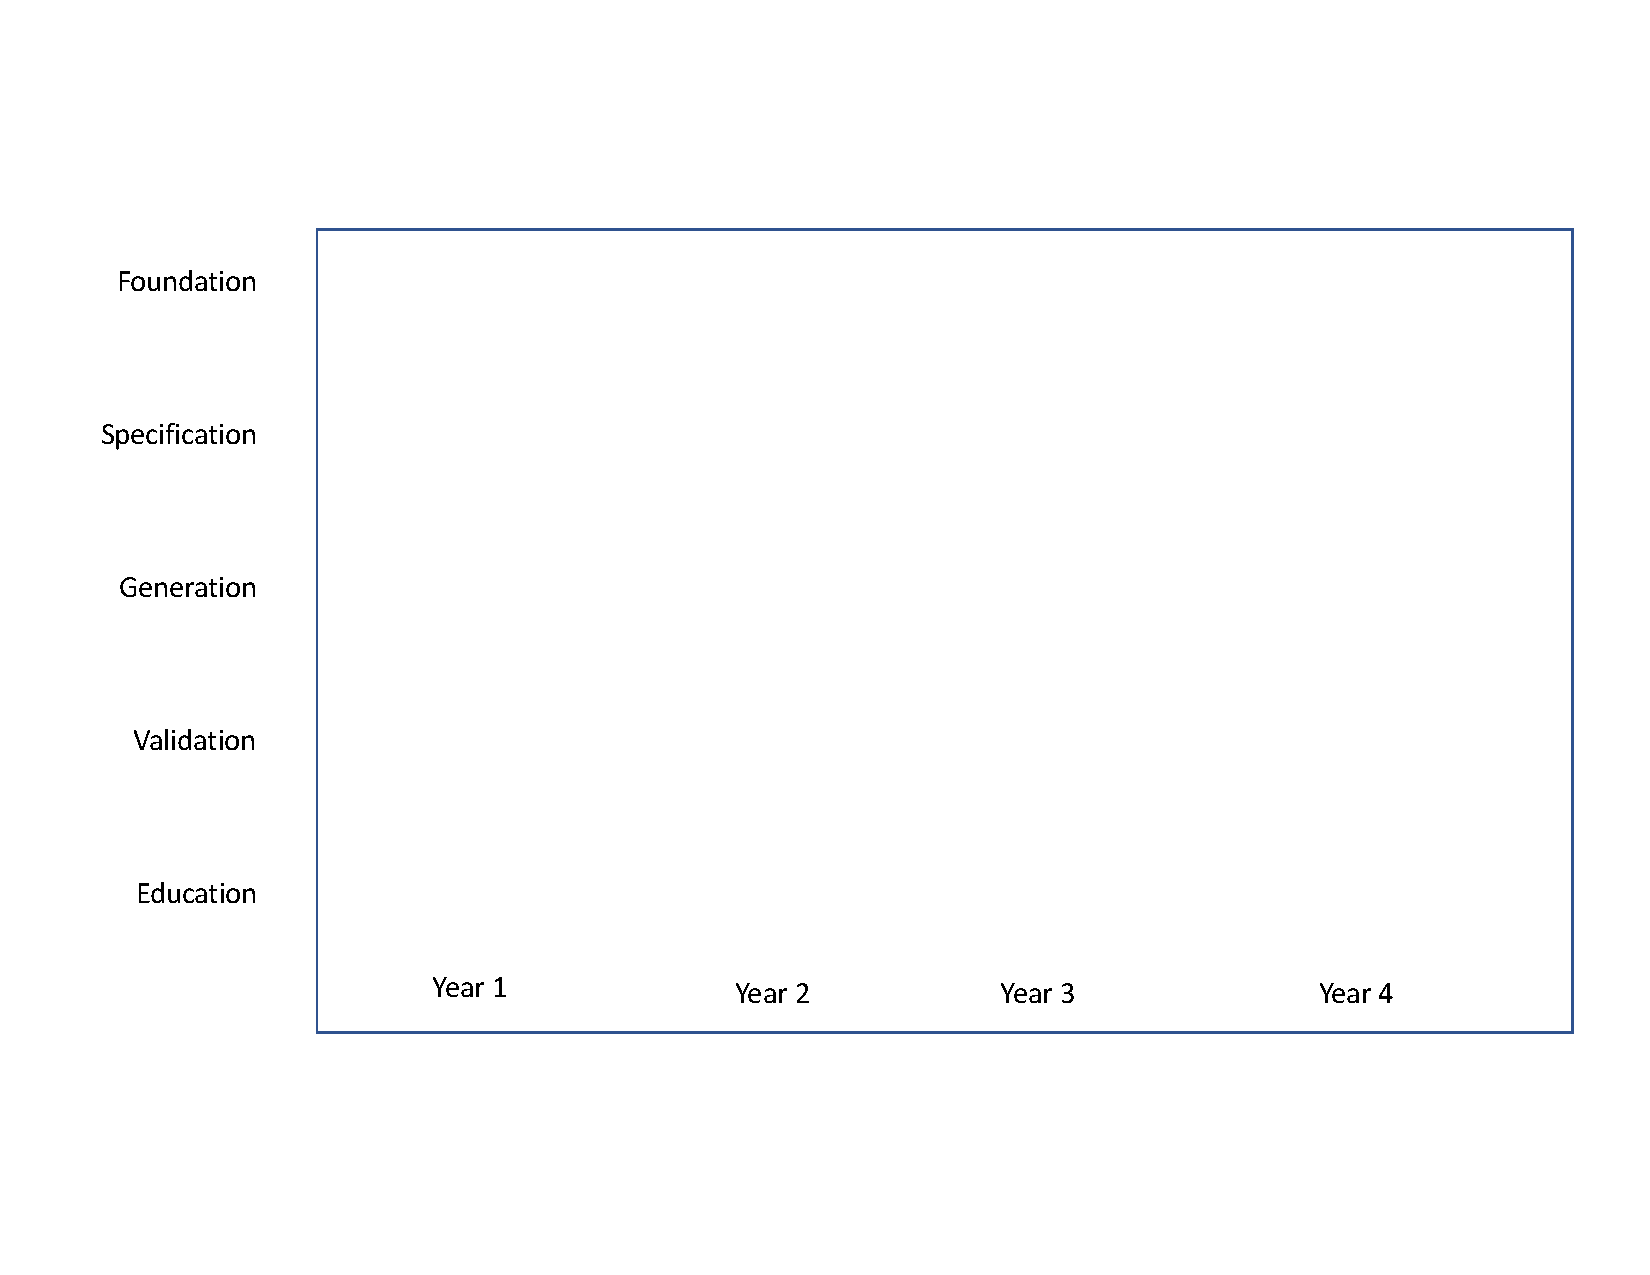
\includegraphics[width=1.1\textwidth]{assets/workplan.pdf}
%   \vspace*{-1.3in}
%   \caption{Plan of work.}\label{fig:workplan}
% \end{figure}

\vspace*{-.3in}

\begin{figure}[ht]
  \centering
\begin{ganttchart}[
      expand chart=\textwidth,
      y unit chart=.4cm,
      %   vgrid
    ]{1}{4}
% \gantttitle{Ongoing}{1}
  \gantttitle{Year 1}{1}
  \gantttitle{Year 2}{1}
  \gantttitle{Year 3}{1}
  \gantttitle{Year 4}{1}
  % \\ \ganttbar
  %      [bar/.append
  %         style={fill=green}]
  %      {\hbox to 3in{\bf Foundation \hfill \footnotesize Task}}
  %      {1}{3}
  % https://www.nsf.gov/pubs/policydocs/pappg22_1/pappg_2.jsp#IIB

\documentclass{NSF}

\graphicspath{{figures/}}

\usepackage{xcolor}
\definecolor{nord-night1}{HTML}{2e3440}
\definecolor{nord-night2}{HTML}{3b4252}
\definecolor{nord-night3}{HTML}{434c5e}
\definecolor{nord-night4}{HTML}{4c566a}
\definecolor{nord-snow1}{HTML}{d8dee9}
\definecolor{nord-snow2}{HTML}{e5e9f0}
\definecolor{nord-snow3}{HTML}{eceff4}
\definecolor{nord-frost1}{HTML}{8fbcbb}
\definecolor{nord-frost2}{HTML}{88c0d0}
\definecolor{nord-frost3}{HTML}{81a1c1}
\definecolor{nord-frost4}{HTML}{5579a5}
\definecolor{nord-red}{HTML}{b14853}
\definecolor{nord-orange}{HTML}{c76d52}
\definecolor{nord-yellow}{HTML}{ebcb8b}
\definecolor{nord-green}{HTML}{69894d}
\definecolor{nord-purple}{HTML}{815679}

\usepackage{listings}
\lstset{
  keepspaces=true,
  mathescape=true,
  frame=none,
  xleftmargin=10pt,
  stepnumber=1,
  belowcaptionskip=\bigskipamount,
  captionpos=b,
  % language=haskell,
  breaklines=true,
  tabsize=2,
  emphstyle={\bf},
  commentstyle=\it\color{cb-blue},
  stringstyle=\mdseries\ttfamily,
  showspaces=false,
  keywordstyle=\bfseries\ttfamily,
  deletekeywords={split},
  columns=flexible,
  basicstyle=\ttfamily,
  showstringspaces=false,
  morecomment=[l]--,
  moredelim=**[is][\color{nord-green}]{@}{@},
  moredelim=**[is][\color{nord-frost4}]{~}{~},
  moredelim=**[is][\color{nord-orange}]{£}{£},
  literate={cP}{{$\mathcal{P}$}}1
  {cG}{{$\mathcal{G}$}}1
  {cGhat}{{$\overline{\mathcal{G}}$}}1
  {cC}{{$\mathcal{R}$}}1
  {cL}{{$\mathcal{L}$}}1
  {fmap}{{$\fmap$}}3
  {[[}{{$\llbracket$}}1 % chktex 9
  {]]}{{$\rrbracket$}}1 % chktex 9
  % {->}{{$\rightarrow$}}2
  % {return}{{$\return$}}6
  % {pick}{{$\pick$}}4
  % {void}{{$\void$}}4
  % {do}{{$\textbf{do}$}}2
  % {>>=}{{$\bind$}}2
  % {<-}{{$\leftarrow$}}2
  % {\\}{{$\lambda$}}1
  % {==>}{{$\implies$}}3
  % {=>}{{$\Rightarrow$}}2
  % {<|>}{{$\langle | \rangle$}}2
}

\newcommand{\citet}[1]{\cite{#1}\todo{fixme}}
\newcommand{\citeauthor}[1]{\cite{#1}\todo{fixme}}

% Macros pilfered from HATRA submission
\definecolor{dkred}{rgb}{0.7,0,0}
\definecolor{dkpurple}{HTML}{4e02eb}
\definecolor{dkgreen}{HTML}{006329}
\definecolor{teal}{HTML}{007982}
\definecolor{string}{HTML}{02782d}
\definecolor{Fuchsia}{HTML}{8C368C}
\definecolor{quoteblue}{HTML}{2264b4}

\newif\ifdraft\drafttrue{}
\newcommand{\comm}[3]{\ifdraft\textcolor{#1}{[#2: #3]}\fi}
\newcommand{\cn}{\ifdraft{\color{blue} [CITE]}\fi}
\newcommand{\bcp}[1]{\comm{dkpurple}{BCP}{#1}}
\newcommand{\hg}[1]{\comm{dkred}{HG}{#1}}
\newcommand{\harry}[1]{\hg{#1}}
\newcommand{\jwc}[1]{\comm{dkgreen}{JC}{#1}}
\newcommand{\amh}[1]{\comm{teal}{AH}{#1}}
\newcommand{\comment}[1]{{\em #1}}
\newcommand{\todo}[1]{{\color{nord-red} TODO: #1}}
\newcommand{\pagebudget}[1]{(#1 pages)}

\newif\iflater\laterfalse

\usepackage{enumitem}

\begin{document}

\title{Property-Based Testing in Practice}
% \title{Property-Based Testing for the Working Programmer}
% \tableofcontents % TODO Remove?
%  BCP - was not working for me, so I followed the instruction to
%  remove :-)
\newpage

% A. Cover Sheet
% A number of the boxes contained on the Cover Sheet are
% electronically pre-filled as part of the FastLane login process
% Complete the rest of your info there

% B. Project Summary
\newsection{B}
\section*{Project Summary}

\todo{``Overview'' needed?}
\subsubsection*{Overview}
Property-based testing (PBT) is an advanced software engineering
methodology where users write executable formal specifications of system
components
and an automated test harness checks these specifications against
many automatically generated inputs.  The bug-finding power of PBT
arises its ability both to work with rich specifications and
to exercise a wide range of system behaviors---both
expected and unexpected---with minimal user guidance.
%
From its roots in the Haskell QuickCheck library, PBT has become
the testing method of choice across much of the functional programming
community; it has also begun to make inroads into industrial practice
at companies such as Quviq, Galois, Stripe, and
Amazon. \forreaders{Any other big companies?  Notable open-source
  projects?}
%
The goal of this proposal is to accelerate this transition
by addressing key challenges in
present-day PBT tools.

What are these challenges?
A need-finding study of PBT at Jane
Street, a Wall Street firm with a focus on software
technology as a competitive advantage, found developers enthusiastic
about its {\em usefulness} but
sometimes frustrated with its {\em usability}.
%
Indeed, the study identified usability as an issue in both major aspects
of PBT methods---{\em specification} of properties and {\em
  generation} of random inputs. Moreover, it revealed challenges
around another aspect of PBT that has so far received less attention from
researchers: how programmers can {\em validate} the
effectiveness of testing.

% At the level of {\em specification}, developers wished for better
% support for expressing common requirements such as ``this
% high-performance implementation of a service must behave exactly the
% same as that reference model'' and for articulating properties of
% poorly modularized code.
% %
% Concerning the other main component of PBT, the {\em generation} of
% random test cases, \todo{...}
% %
% Developers also need better {\em validation} tools for checking
% that their testing is actually effective.\todo{blah}
% %
% Finally, better {\em education} of potential PBT users is critically
% required.

% \amh{How about the following framing? In this project, we define a practice of
% usable property-based testing, and conduct foundational research in PL and HCI
% to bring about this practice. We define usable property based-testing as having
% two main components. First, providing visibility into what can be extremely
% complex test outcomes. Second, supporting the efficient expression of
% tests.\ldots{} And then we can jump into talking about the challenges that we
% plan to solve in specification, generation, validation, and education.}.
% %
% At the level of {\em specification}, developers wished for better
% support for expressing common requirements such as ``this
% high-performance implementation of a service must behave exactly the
% same as that reference model'' and for articulating properties of
% poorly modularized code.
% %
% Concerning the other main component of PBT, the {\em generation} of
% random test cases, \todo{...}
% %
% Developers also need better {\em validation} tools for checking
% that their testing is actually effective.\todo{blah}
% %
% Finally, better {\em education} of potential PBT users is critically
% required.

%  and ``shrinking'' of failing
% tests to minimal counterexamples,

To make PBT more usable, two largely disjoint
research areas must be
brought to bear.  PBT itself is grounded in domain-specific languages
and formal methods---traditional topics in the field of Programming Languages.
Usability, on the other hand, is the domain of Human-Computer Interaction.
%
This four-year project will combine insights, methods, and tools from
PL and HCI to advance the usability of PBT along all three of its
axes---specification, generation, and validation\iflater\todo{We may
  need to reorder these, depending on what happens with the global
  structure.}\fi---and bring it to a
broad community of software developers.

\smallskip

\noindent{\bf Keywords:} Programming languages; human-computer
interaction; property-based testing; usability.

\subsubsection*{Intellectual Merit}
The project will advance knowledge along four interconnected axes.
%
First, it will establish a firm {\bf\em foundation} for HCI-informed
research on PBT, supplementing past and ongoing user studies with
broader surveys of PBT across the software industry and real-time
observations of developers interacting with PBT.
%
Second, it will offer developers more usable {\bf\em specification} tools,
including a language for stating temporal properties over internal
program states and automation for model-based testing of
modular abstractions.
%
Third, it will explore a novel abstraction for random input {\bf\em
  generation} that enables a range of use cases---generating inputs
satisfying validity conditions, mutating inputs to explore the space
of similar inputs, and manually or automatically tuning a random
generator's distribution based on examples or code coverage.
%
And fourth, it will develop new interactive tools for rapid {\bf\em
  validation} of the effectiveness of testing, for helping programmers pin
down the causes of failures, and for visualizing generated data
distributions to support comprehension and tuning.

%  (1) deploy tools from HCI to better
% understand the challenges to wider adoption of PBT, (2) combine PL and
% HCI methods to build solutions, and (3) develop educational materials
% to make PBT concepts and tools accessible to a broad community of
% university students and industrial developers.

\subsubsection*{Broader Impacts}
A fifth thread of activity, coordinated with the rest and integral to the
project's aims, will be advance {\bf\em education} in PBT in both universities and industry. We will
develop materials for teaching industry programmers how to identify
high-leverage situations for using PBT, curricula for teaching mature
and powerful PBT practices to undergraduate students, and tooling to help
PBT beginners write their first properties.
%
A general-audience article on PBT for CACM will also help broaden the
reach of PBT.

Work on the project will include and elevate undergraduate
researchers, including some from diverse backgrounds that will be
funded through a new NSF-REU. These undergraduates will work
closely with the two PIs and four Ph.D.{} students in an interconnected and supportive
research environment.

The ultimate goal, through education, publications, and open-source
tools, is to make property-based testing a standard tool on every
software developer's testing toolbelt.  Better testing, in turn, will
lead to software systems of every sort that are less expensive, more
robust, and more reliable.


% The statement on broader impacts should describe the potential of the proposed activity to benefit society and contribute to the achievement of specific, desired societal outcomes.


% C. Table of Contents
% A Table of Contents is automatically generated for the proposal by FastLane

% D. Project Description
\newpage\newsection{D}
\section{Project Description \pagebudget{.5}}

\comment{Meta comment: I think a lot of the technical content here can come from my thesis proposal. It has all of the technical projects other than the benchmarking project (which BCP should be able to write about — or maybe ask for Jessica’s help?) and it also has the background and related work. It may be useful to go to the individual papers for some deeper details, but I’d be surprised.}

\todo{Harry proposal page 4 and 6.5-8}

\todo{
[MODEL AFTER THESIS INTRO / CONCLUSION]
\begin{itemize}
   \item High level: Advance the theory and practice of PBT, making it more valuable to a wider range of software engineers
   \item PBT is great
\begin{itemize}
      \item For people who like formal methods, it’s a way to write a formal spec and check it without doing full verification
      \item Even for people who don’t, it’s been extremely effective finding bugs in practice
         \item Cite…
      \item (?) And people really like it (maybe pull quotes from preliminary study)
\end{itemize}
   \item But there is still room for PBT to grow (maybe stats, feel free to refine this argument more)
   \item We want to advance the theory and practice of PBT so it is more valuable to SEs
\end{itemize}
}

\subsection{Background and Related Work \pagebudget{1.5}}

\subsubsectionstar{PIs' Prior Qualifications}

\subsection{Extending the Foundation \pagebudget{3}}

\todo{
\begin{itemize}
   \item Story
\begin{itemize}
      \item The research community has identified that random generation (and in particular, the valid generation problem)[b] causes problems for testers
      \item This shows up in prior work, and also in realistic examples (e.g., the fuzzing community really cares about this!)
      \item We’ve already done some work to explore new abstractions for random generation (free generators) and we have more that we want to try (reflective generators)
      \item In addition, the PBT community is missing tools to empirically evaluate generation strategies
      \item And the PBT literature is also woefully disconnected from the fuzzing literature, where they have their own partial solutions to this problem
\end{itemize}
   \item Prior Work - Free generators [CHAPTER 1[c] OF THESIS PROPOSAL is a
   source, but it's way too long -- we need to write a compact precis of the
   crucial points]
   (perhaps also some other prior things)
   \item Planned Work - Reflective generators [CHAPTER 2 OF THESIS PROPOSAL]   (needs new work on evaluation; maybe rests on benchmarking infrastructure; validity-preserving mutation scheme needs to be evaluated by real implementation and measurement)
   \item Planned Work - Empirical Evaluation Playground [JESSICA OR BENJAMIN WRITE] (can ultimately be used for Benchmarking; in the short term, it’s a playground for individual PBT efforts to see how they are doing)
   \item Speculative Work - Add PBT incrementally to a fuzzing system [CHAPTER 3 OF THESIS PROPOSAL](follows directly from the free and reflective generators work)
\end{itemize}
}

\subsection{Finding out what working programmers need \pagebudget{3}}

\todo{
\begin{itemize}
   \item Story
\begin{itemize}
      \item The projects above follow the lead of prior work, solving problems that have already been identified, but we have no reason to believe that those problems are exhaustive
      \item Indeed, there may be high-leverage opportunities to improve PBT that have nothing to do with the valid generation problem
      \item We’re in the process of uncovering “unknown unknowns” by talking to PBT users about their experiences - we’ve already done a preliminary study, and we plan on talking to Jane Street developers for a full-scale study
      \item We’re not sure what we should do after that, but the preliminary study gave us some ideas
\begin{itemize}
         \item We can obviously keep talking to users (via surveys or observations)
         \item We also identified that there are likely workflow improvements that could help PBT fit into a developer’s environment better (and user-centered design opportunities there)
         \item We may even find interesting PBT opportunities at Jane Street that will give us a hands-on opportunity to solve problems that real developers are actively dealing with
\end{itemize}
\end{itemize}
   \item Prior Work - Pilot study [CHAPTER 4 OF THESIS PROPOSAL / HATRA]
   \item Planned Work - Jane Street Study [CHAPTER 4 OF THESIS PROPOSAL / HATRA]
\end{itemize}
}


Part 1 of the ``unknown unknowns''.
Jane Street study, preliminary study, observations, surveys.

In this aim, we plan to set course for research in PBT, both broadly and for the
future directions of our group. We will conduct a series of formative studies,
each addressing one of three main goals:

\subsubsectionstar{Understanding Challenges to Using PBT Tools}

The first step is to conduct qualitative interviews to understand the challenges
that programmers face when using PBT tools.

Here I will elaborate on the design of the Jane Street study.

\subsubsectionstar{Characterizing the Potential Reach for PBT Tools}

We will conduct a survey with the purpose of understanding the impact that
improved PBT tools could have in industry, if major usability issues were
addressed. We see this survey as crucial in understanding the amount of
resources that should be devoted to PBT research. Furthermore, this
questionnaire will help shed light into which of the usability challenges from
the interview study, if addressed, are most likely to impact a broad set of
current and prospective users of PBT tools.

\subsubsectionstar{Understanding the Structure of PBT Tasks in Detail}

The next step is to more deeply characterize the obstacles faced with specific
tools and tasks through close observation. We anticipate conducting observations
of participants formulating properties and creating generators, as we expect
that close observation of developers performing these tasks will yield yet
additional detail about ways that developers are supported and not supported by
the tools they use today to a level of depth we will not achieve with the
interviews.

\subsection{Exploiting the Foundations to Build Powerful, Interactive PBT Tools \pagebudget{3}}

Upon the advanced technical foundation from Aim 1 and the refined understanding
of programmers' needs from Aim 2, our final aim (Aim 3) will focus on the
development of programmer-facing tools that allow them to leverage properties in
testing their code more efficiently and effectively.

While the specific focus of our tool design and research efforts will be
continually refined on the basis of what we learn from Aim 2, below we detail
several directions that we expect to lead to the design of tools that are both
innovative within the research community, as well as potentially impactful,
drawing on the lessons learned from the preliminary need-finding research we
have done to date as well as our own intuitions, and as critical users and
engaged members of the communities for these tools.

\todo{Discuss:

\begin{itemize}

% \item Some of the tools we propose in this section may depend on a technical
% background we do not have on this team. For instance, property generation.
% Should we be keeping the scope of the proposed work to those where we as a team
% have expertise in the backend technologies? After discussing with BCP, we need
% not limit ourselves to areas where we are at present the leading experts. Let's
% draft the descriptions, see the ones we are excited about, wave away some
% of the details that we have not yet educated ourselves, and go from there.

\item We should ask Jane Street for a letter of support indicating their
willingness to collaborate on the need-finding activities.

\end{itemize}
}

\subsubsectionstar{Interactive property specification}

Developers in the preliminary interview study indicated that while they knew their software would benefit from property-based testing, sometimes they had difficulty imagining which properties to test. One area that could benefit from innovation in PBT tools is in designing tools that help programmers imagine properties in situations like these.

To date, research has shown the potential for automated tools to extract invariants describing a program's behavior\cite{ammons2002mining,le2018deep,claessen2010quickspec}. However, the integration of such tools into developer workflows is non-trivial. We posit that a usable tool that can help with imagining properties would need the following features:

\textit{Readable code generation}. While prior techniques have succeeded in generating invariants, we expect that users of PBT systems would benefit from having properties generated in the language of their property-based testing tools. Furthermore, there are some variants about systems that may be so complex that they require significant comprehension time for users (i.e., those involving a large number of clauses). In such cases, a tool may way to generate simpler variants of properties first, and allow developers to refine them on their own.

\textit{Generating important properties}. Non-trivial programs can be described by an overwhelmingly large number of properties, many of which describe only incidental aspects of the program's behavior that do not need to be tested. How can tools produce those properties that developers would want to have tested? We believe that this is a problem that can be best solved with a mixed-initiative approach~\cite{allen1999mixed}---that is, judiciously incorporating both developer input and automation. Developer could guide a specification mining tool to extracting relevant properties through input mechanisms such as (1) identifying regions of code that are likely to lead to an adverse behavior such as an exception or a logical error; (2) providing unit test cases that test a special case of a generalized property; and (3) indicating aspects of interest on input and output data during exploration in a debugging REPL.

\textit{Property refinement}. Tools could help a developer refine generated properties. If a generated property is too relaxed, the tool could request that developer provides a counterexample that should trigger a failure, and then regenerate the property. If a generated property is too strict, a tool could allow a programmer to mark a counterexample that was generated by the PBT tool as spurious, i.e., not indicating an actual failure of the program. In each of these cases, the property generator may have generate multiple properties for a developer to review, each of which may satisfy the refinements that a developer has provided.

\textit{Plan of work}: Incorporating known, widely-used specification mining tools such as QuickSpec~\cite{claessen2010quickspec}\ldots{}

% One challenge identified by software developers we have spoken with is that it can be difficult to come up with a property to test with property-based testing tools. Perhaps tools could help programmers come up with, and express, properties that they wish to be tested. To design such tools, we will adapt techniques from the specification mining literature to generate candidate properties (e.g.,~) and interfaces that help programmers select from, and refine, generated properties.
% 
% A first step will be to generate candidate properties. These will be generated using specification mining techniques. Specifications will need to be mapped from an abstract representation of the property to an expression of that property in the programming language, such as Hypothesis' property specification language. A major challenge is that a specification mining technique will produce many spurious properties which do not describe aspects of the program that the programmer wishes to test. Affordances will be added to the programming environment to allow a program to select subsets of code that manipulate properties of interest; and to generalize from behaviors that are implied by individual unit tests, or observations made during debugging, to greatly limit the space of generated properties.
% 
% A second step will be to assist in the refinement of properties. In some cases, generated properties will be too broad; for instance, . if the testing tools yield a counterexample, the counterexample may be an indicator that a property is insufficiently strict, rather than an indication that the program is incorrect. @Andrew, continue from here\ldots{}
% 
% Motivation: Informants struggled to figure out what to test. informants had an intuitive idea of what “right” and “wrong” was. Perhaps they could have been helped with a tool that refined that expectation into something that was formal.
% 
% Plan of work: A first step in this process might be a tool that refines a wrong specification that has some counterexamples into a clean, correct specification. When a counterexample is encountered, you can fix the program if it represents a bug, or you will have to refine a property if the property was not written correctly.
% Alternatively, a greenfield specification maker might depend on a machine learning backend. We need to know more about how this works. Perhaps speak to Mayur about unit test generation. The tool design would focus on coming up with usable property specifications, and potential some user input (e.g., pointing to parts of programs that should be involved in property creation). Could specifications be provided as natural language? QuickSpec works okay for Haskell using static analysis to determine invariants. We would need someone with ML or program synthesis background to work on this project.
% 
% Example: For a serialization / deserialization pair of functions, testing that the serialized deserialized string is the same version as the original string; the refinement is to exclude Unicode strings, which do not have to be supported by serialization functions.

\subsubsectionstar{Visualizing and tuning data distributions}

% (this topic is what Joe is most excited about)

% For visualizing data distributions...

Plan of work: easily computable summary statistics; as well as user-defined metrics for understanding what you care the most about from the distribution. Seeing what the “average” data structure is that is getting generated. For multimodal data, what are the different modes of data. The set of data types to be handled in PBT are: algebraic data types, lists, trees (this would also cover programs). Joe thinks we already have good visualizations for numbers, booleans, and strings; it is compositional data types that we lack good visualizations for. People need to (1) see representative examples (2) understand spread (3) indicate areas of the space that should not be explored.

% For tuning data distributions...

Plan of work: indicating areas of the distribution that should not be generated.

Example: writing a generator of programs (for instance, to test out a compiler). You want lots of different programs that make sense in different ways. You want large ones, small ones, ones that use variables in coherent ways, ones that don’t overuse certain constructs, ones that use a variety of different language features. You want the generated programs to be representative of those that people might write. You also want some weird programs to catch the edge cases, but you don’t want all weird programs. (How big, how deep, how wide of programs?). Also, for trees, one might want to specify heights and breadths of the tree.

\subsubsectionstar{Debugging support for understanding counterexamples}

Once a PBT tool generates a counterexample of where a property fails, a programmer will need to understand what in an input caused the program to fail. This task can be rather challenging because generated inputs can be complex, deep data structures \todo{Do we have a reference that implies the complexity of generated counterexamples?}. Methods for making it clearer why a counterexample fails could be to generate additional inputs that are very close to the counterexample that are actually correct, to run the program up to the point where the traces of the programs begin to diverge, and then to drop a programmer into a debugging environment where they can query the state of the program and step through the remainder of the execution. PI Head has prior work designing debugging tools that help programmers understand trace divergences in an educational setting~\cite{suzuki2017tracediff}.

\subsubsectionstar{Reconciling generator API design with imperative language idioms}

Motivation: How do you design a generator DSL in an imperative language? A generator uses higher-level functions in a way that might be confusing to people who used Python.  (e.g., passing a generator of numbers to a generator of lists to get randomized lists of numbers). Is there a way of designing APIs for generators that can make the composition of these types of generators easier to reason about and express for some programmers?

(Joe says the DSLs are well-designed, but the code is hard to debug. How do you write a generator that works really well, that has a good data distribution and finds bugs? See below.)

Plan of work. Not sure. This might require some discussions with more uses of Hypothesis-like libraries.

Next steps—get examples of sloppily-expressed PBtests in Python and then think through how they would be written more clearly.

\subsubsectionstar{Integration with continuous integration workflows}

\todo{Section 6.2 of Harry's thesis proposal.}

\subsubsectionstar{Tailoring PBT for financial systems}

I am not sure what should go here. I am a bit wary of focusing specifically on developing tools for financial systems if the focus of this grant proposal is to make PBT tools more broadly useful.

\subsection{Education \pagebudget{1}}

\subsection{Plan of Work \pagebudget{.5}}

\subsection{Broader Impacts \pagebudget{.5}}
The Project Description must contain, as a separate section within the narrative, a section labeled ``Broader
Impacts of the Proposed Work". This section should provide a discussion of the broader impacts of the proposed
activities. Broader impacts may be accomplished through the research itself, through the activities that are
directly related to specific research projects, or through activities that are supported by, but are complementary to
the project. NSF values the advancement of scientific knowledge and activities that contribute to the
achievement of societally relevant outcomes. Such outcomes include, but are not limited to: full
participation of women, persons with disabilities, and underrepresented minorities in science, technology, engineering, and
mathematics (STEM); improved STEM education and educator development at any level; increased public
scientific literacy and public engagement with science and technology; improved well-being of individuals in
society; development of a diverse,globally competitive STEM workforce; increased partnerships between
academia, industry, and others; improved national security; increased economic competitiveness of the United
States; and enhanced infrastructure for research and education.

\subsection{Results from Prior NSF Support \pagebudget{.5}}
If any PI or co-PI identified on the project has received NSF funding (including any current
funding) in the past five years, in formation on the award(s) is required,
irrespective of whether the support was directly related to the proposal or not.
In cases where the PI or co-PI has received more than one award (excluding amendments),
they need only report on the one award most closely related to the proposal. Funding includes not just salary
support, but any funding awarded by NSF. The following information must be provided:\\

\noindent
\emph{\underline{Name of PI}}: NSF-Program (Award Number) ``Title of the Project'' (\$AMOUNT, PERIOD OF SUPPORT).
{\bf Publications:} List of publications resulting from the NSF award. A complete bibliographic citation for each
publication must be provided either in this section or in the References Cited section of the proposal); if
none, state: ``No publications were produced under this award.'' {\bf Research Products:} evidence of research products
and their availability, including, but not limited to: data, publications, samples, physical collections, software,
and models, as described in any Data Management Plan.

% \subsubsection{Proposed Study}
% The Project Description should provide a clear statement of the work to be undertaken and must include:
% objectives for the period of the proposed work and expected significance; relation to longer-term goals of the PI's
% project; and relation to the present state of knowledge in the field, to work in progress by the PI under other
% support and to work in progress elsewhere.
%
% The Project Description should outline the general plan of work, including the broad design of activities to be
% undertaken, and, where appropriate, provide a clear description of experimental methods and procedures.
% Proposers should address what they want to do, why they want to do it, how they plan to do it, how they will
% know if they succeed, and what benefits could accrue if the project is successful. The project activities may be
% based on previously established and/or innovative methods and approaches, but in either case must be well
% justified. These issues apply to both the technical aspects of the proposal and the way in which the project may
% make broader contributions.

\subsection{More stuff to not forget :-)}

Unfunded collaborations: Any substantial collaboration with individuals not included in the budget should be described in the Facilities, Equipment and Other Resources section of the proposal (see Chapter II.C.2.i) and documented in a letter of collaboration from each collaborator. Such letters should be provided in the supplementary documentation section of FastLane or Research.gov and follow the format instructions specified in Chapter II.C.2.j. Collaborative activities that are identified in the budget should follow the instructions in Chapter II.D.3.

Remember to not use any URLs in the project description!  (They are
encouraged in the references.)


% E. References Cited
\newpage\newsection{E}
\renewcommand\refname{References Cited}
\bibliography{andrew,harry,bcp}
% I prefer to use the IEEE bibliography style.
% That's  NOT required by the NSF guidelines.
% Feel Free to use whatever style you prefer
% \bibliographystyle{ACM-Reference-Format}
\bibliographystyle{IEEEtran}

% F. Biographical Sketch(es)
\newpage\newsection{F}
See here for advice on how to write these:
\url{https://www.nsf.gov/bfa/dias/policy/disclosures_table/june2021.pdf}

% G. Budget Justification
\newpage\newsection{G}
\iflater
\section*{Budget Justification}

\todo{GPG: Budgets for all projects must include funding for one or
  more designated project representatives (PI/co-PI/senior researcher
  or NSF-approved replacement) to attend each annual PI meeting during
  the proposed lifetime of the award.}

\todo{GPG: a portion of the budget for each Core Programs, Large
  Projects proposal may be used to engage relevant Broadening
  Participation in Computing (BPC) expertise to help plan, organize,
  coordinate and execute BPC activities.}

\todolater{Make sure to account for PhD months accurately---note when
  people start.}

\hg{Any chance we want to budget for a new machine for someone (e.g., one or
more of the potential other PhD students)? Or is that priced in?}
\bcp{Good catch -- yes, we want to budget for new machines for all.
  Possibly also a server, for running lots of tests faster...}

\todo{REPL students (see comments here)}
% And attached is the budget sheet from PEFS. The TLDR yearly costs are….

% Direct Student Costs
% ================
% Travel - $400 per student per year
% Housing - $2500 per student per year
% Stipend - $6000 per student per year

% Indirect Student Costs
% =================
% Admin - $32,500 per year (10k for lead admin, 10k distributed across PLClub+ leaders, with Penn’s 62.5% overhead stacked on top)

% Let me know if you have any questions. If you want to contribute to indirect student costs, I’m not totally sure what the right amount is — but it seems we’re currently charging about $4,000 per student per year in admin costs.

\discuss{Should we be asking for budget for a compute server or AWS or
  any other Cloud Computing service (e.g., NSF itself has one)), for
  running heavy testing workloads??  If not, we should say so.  The
  benchmarking project, for example, could use this!}

% No more than 3 pages!!!
\subsection*{A. Senior Personnel}
\noindent{\bf A1.} Includes two PIs at 18\% CY.
\subsection*{B. Other Personnel}
\noindent{\bf B3.} Includes stipend for one graduate student for each calendar year of the project.

\todo{Webinar: Staff support is normal.  Needs to justified not only
  in the body of the proposal but also carefully called out in the
  budget justification.}

\subsection*{C. Fringe Benefits}
Fringe benefits are calculated at a rate of X\% for faculty, Y\% for graduate students.
\subsection*{E. Travel}
1) all travel (both domestic and foreign) must now be justified.
2) temporary dependent care costs above and beyond regular dependent care that directly result from travel to conferences are allowable costs provided that the conditions established in 2 CFR § 200.474 are met.
\subsection*{G. Other Direct Costs}
1) Includes coverage on costs of computing devices
2) The charging of computing devices as a direct cost is allowable for devices that are essential and allocable, but not solely dedicated, to the performance of the NSF award
\noindent{\bf G5.} Includes tuition for graduate students participating in the program.
\subsection*{H. Indirect Costs}
Overhead at a rate of X\% is charged on all direct salaries and wages, applicable fringe benefits, materials and supplies, services, travel and subawards up to the first \$X of each subaward. Excluded are equipment and the portion of each subaward in excess of \$X.
\fi


%  H. Current and Pending Support
\newpage\newsection{H}
\section{Current \& Pending Support}
\begin{tabular}{ll}
\textbf{Investigator:} 			& \\
\textbf{Project Title:}			& Put your Proposal title here\\
\textbf{Project Location:}		& \\
\textbf{Source of Support:} 	& NSF\\
\textbf{Total Award Amount:} 	& \\
\textbf{Total Award Period:}	& \\
\textbf{Status:}				& Pending (this project) \\
\end{tabular}


% I. Facilities, Equipment and Other Resources
\newpage\newsection{I}
\section*{Facilities, Equipment, and Other Resources}

Penn's departmental computing facilities include a standard collection of
networking services, printers, fileservers, and compute servers.  No
specialized facilities or equipment will be needed to carry out the
proposed work.

\todo{Mention, here, any machines we've budgeted for in the budget
  section?}

\hg{Other things off the top of my head then: travel for speaking, meetings, and
conferences (lots), REPL funding (talking to Joey next week), desk setups for
the new students, a bit of money for hosting PBT-focused PLClub speakers? ---
I'm just guessing at stuff, just take the parts that make sense}

\discuss{
Document all three (four?) unfunded external collaborations.
  \begin{itemize}
  \item Any substantial collaboration with individuals not included in
  the budget should be described in the Facilities, Equipment and
  Other Resources section of the proposal (see Chapter II.D.2.g) and
  documented in a letter of collaboration from each collaborator. Such
  letters should be provided in the supplementary documentation
  section of Research.gov and follow the format instructions specified
  in Chapter II.D.2.i. 
  \item We also need to make sure that the appropriate sections of the
  project description mention the collaborations.
  \end{itemize}
}





% J. Special Information and Supplementary Documentation
\newpage\newsection{J}
\section*{Data Management Plan}

The project will produce four types of data.

\begin{enumerate}
\item Software artifacts,
including implementations, test cases, software revision histories, and
other items.  These will be distributed under an open-source
license.  They will be documented so as to allow others to understand,
use, and modify them.  (Both PIs have extensive records of
distributing artifacts in this way.)  Artifacts will be made available
to the public on Github and maintained for at least three years beyond
the end of the project lifecycle.

\item Technical papers and talks describing our experiences
and results.  These will be published in academic conferences and journals.
Drafts will be made available on Arxiv.

\item Educational materials aimed at undergraduates, masters students,
and professional developers, which will be made available on the
project's public website under an open-source license.

\item Raw data gathered during user studies, which will be kept
confidential and stored securely in accordance with IRB-approved best
practices.
\end{enumerate}

\iflater{%
\amh{Consider integrating the following, which Andrew wrote up for his NSF
CAREER to address more of the concerns the data management plan is asked to
address.}

\paragraph{Data from usability evaluations} As part of routine tool design and
evaluation activities, we will collect human subjects data in the form of questionnaire responses, interface usage
logs, and, during lab evaluations, screen recordings, audio recordings, and
researcher notes. Data will be collected from users in the following settings: (1)
in-lab usability studies; (2) interviews and observations with expert authors;
(3) instructor usage of the tools to augment instructional materials in CIS 545 and CIS 421; (4) student
use of augmented documents in the same classes; and (5) usage of the
tools in the wild.

All data from human subjects will be collected, stored, and analyzed in accordance
with institutional best practices following procedures that have undergone review by Penn's Institutional
Review Board. In all circumstances, users' express consent will be obtained
prior to collection and analysis of data. Data will be handled in a way that is sensitive
to the following considerations:

\emph{Confidentiality}. User confidentiality will be preserved by collecting
only those identifiers absolutely necessary to manage studies and conduct the required
analyses. Identifiers that need to be collected will be removed from the data when it
becomes possible to do so: for instance, audio recordings will be transcribed and then
deleted to remove the identifier of participants' voices, and identifiers (like
names and company affiliations) will be removed from transcripts. Participants will
be able to request that we delete or redact usability data should it contain information that is sensitive for them. Any transcription services that we use will have signed strict confidentiality agreements.

\emph{Security}. Human subjects data will be collected, stored, and analyzed on password-protected,
encrypted machines managed by research personnel who have undergone human subjects research
training. The data may also be stored on secured departmental servers and password-protected
shared folders hosted in university-approved cloud services.
We will retain data long enough that the Ph.D. student researcher can consult it throughout their entire program of study. Our plan is to retain study data for seven years following the project start date. After that time, the data will be deleted.
}
		% Data Management Plan (Required)
%\input{sections/postdoc} % Postdoctoral Researcher Mentoring Plan (if applicable)

\end{document}

\end{ganttchart}
  \caption{Plan of work.
   % \bcp{The timeline needs to be brought into correspondence with our
   %   actual expectations of timing, and explained.  Harry's projects
   %   should end by year 3 latest!  :-)}
   % \hg{How's that?}
   % \bcp{Hmm---now it looks like there's not much happening in year 4!
   % Maybe we need to remove this constraint.  Also, there's not much
   % blue at the moment, and I'm not certain how to talk about the
   % distinction between the two students' domains of work.  Can we try
   % to make it more coherent (even at the cost of some accuracy
   % wrt. our expectations about what you're going to do)?}
}\label{fig:workplan}
\end{figure}

The work of the project will be carried out by two PhD students (and
a number of undergraduates or masters students), over the course
of four years.  All the work will be collaborative across the group,
but the specific threads can be roughly divided into two broader
thrusts, one focused on PL techniques (advised by PI Pierce) and the
other emphasizing HCI methods and tools (advised by PI Head).

The PL thrust, likely led by PhD candidate Harrison Goldstein, will be
concentrated in years 1--3 (see the blue bars in
Figure~\ref{fig:workplan}).  This student will first finish the work on
reflective generators and write the {\em When to Specify It!} survey;
later on, they will consider reflective shrinkers and fuzzers,
collaborate with the other PhD student on tools for tuning data
distributions, and advise undergraduates and masters students on
languages for writing properties over logs and on automation for
testing ML modules.  (Goldstein has a proven track record of advising
and co-advising junior students---e.g.,~\cite{pytestmutagen}.)

The HCI thrust will likely be the responsibility of a new PhD student,
hired in year 1 or 2; this thread of work will thus be concentrated in
years 2--4 (shown in yellow in Figure~\ref{fig:workplan}). This thread
will include formative HCI research--- surveys to generalize our
motivating study and observations of PBT in practice---as well as
human-centered design projects including tools to validate data
distributions, interactive shrinking and debugging, and interactive
property specification. The second student will also co-advise an
undergraduate or masters project centered around turning
counterexamples into regression tests.

The work on incorporating PBT in the undergraduate curriculum (shown
in green) will involve both students equally and will evolve over the
course of the four year project.

\SIMPLESECTION{Broader Impacts of the Proposed Work%
 \pagebudget{.5}}{sec:broader-impacts}

\paragraph*{Educational Benefits}
%
The most immediate broad impact of the proposed work will be the
development of educational materials. Educational activities will be
coordinated with the rest of the work, and they are integral to the
project's overall goal of making PBT a standard testing methodology,
readily available to every industrial developer.  Specific pedagogical
threads within the project are described in~\sectionref{sec:ed}.

The majority of requested funding will support graduate students.  We
also plan to work with undergraduate students during this project;
they, too will benefit from the research experience. Each graduate
student will have leadership responsibility for multiple facets of the
project, including co-supervising interested undergraduate
researchers.

Our research group is already relatively diverse---PI Pierce has one
female Ph.D.{} student (who may, indeed, be interested in this
project) and PI Head has two---and we will continue pushing to make it
more so.  Pierce (along with Penn colleagues Zdancewic and Weirich)
was also recently informed that he will likely receive funding for an
NSF REU program that will involve 24 undergraduates in research (8 per
year for three years), selected specifically with an eye to diversity;
some will certainly end up working on this project.
See the appendix on Broadening Participation in Computing for more
details.

\paragraph*{Benefits to Society}
%
The project's goals will also be served by open-source distribution of
all of the tools built during the project.  We hope to engineer these
to a standard that will make them directly useful to engineers and
students; more importantly, though, they will serve as models for
similar tools for other programming languages and environments.

The project also represents an excellent opportunity for collaboration
between university researchers and industrial advocates of PBT.  Our
ongoing user study at Jane Street has been carried out with the
enthusiastic support of their developers and management, and we hope
to continue using them as a testbed for prototypes of the tools we
will build.  Similarly, we are in active discussions with the
developers of the Hypothesis testing tool for Python, who are keenly
interested in the results of the survey study described in
\sectionref{sec:survey}.

Longer term, better testing means better software.  As software
systems have grown to the gigantic scale seen today, good testing
methodologies and tools (unit testing tools, test-first design
methods, etc.) have come to play an ever more crucial role.  Adding a
powerful new testing tool to programmers' arsenals will further boost
this part of the development process, leading to software of every
sort that is more robust, more reliable, and less expensive to build.


% \proposecut{See the Collaboration Plan for
% more.}

% The Project Description must contain, as a separate section within the narrative, a section labeled ``Broader
% Impacts of the Proposed Work". This section should provide a discussion of the broader impacts of the proposed
% activities. Broader impacts may be accomplished through the research itself, through the activities that are
% directly related to specific research projects, or through activities that are supported by, but are complementary to
% the project. NSF values the advancement of scientific knowledge and activities that contribute to the
% achievement of societally relevant outcomes. Such outcomes include, but are not limited to: full
% participation of women, persons with disabilities, and underrepresented minorities in science, technology, engineering, and
% mathematics (STEM); improved STEM education and educator development at any level; increased public
% scientific literacy and public engagement with science and technology; improved well-being of individuals in
% society; development of a diverse,globally competitive STEM workforce; increased partnerships between
% academia, industry, and others; improved national security; increased economic competitiveness of the United
% States; and enhanced infrastructure for research and education.

\SIMPLESECTION{Results from Prior NSF Support\pagebudget{.5}}{sec:prior}

% If any PI or co-PI identified on the project has received NSF funding (including any current
% funding) in the past five years, in formation on the award(s) is required,
% irrespective of whether the support was directly related to the proposal or not.
% In cases where the PI or co-PI has received more than one award (excluding amendments),
% they need only report on the one award most closely related to the proposal. Funding includes not just salary
% support, but any funding awarded by NSF. The following information must be provided:\\

\emph{\underline{PI Pierce}}: (NSF 1955565) ``Collaborative Research:
SHF: Medium: Bringing Python Up to Speed'' (\$437,999,
7/2020--6/2023), with co-PIs Michael Hicks (Maryland) and Emery Berger
(Amherst).
The project aimed to dramatically increase the performance and
correctness of applications written in Python by developing novel
techniques for performance analysis, optimization, run-time systems,
property-based random testing, concolic execution, and program
synthesis. It developed both
novel performance analysis tools and optimizations and novel automatic
testing frameworks. These were largely tailored to and implemented for
Python, but applicable in other, similar languages.
%
{\bf Intellectual Merit.} The project involved work on both
performance measurement (mostly at Amherst and Maryland) and PBT (mostly at Penn
and Maryland).  Specific threads of work involving Penn included
building an early
version~\cite{Frohlich2022} of the Reflective Generators described in
\sectionref{sec:reflective}, carrying out the pilot study of PBT in Python
mentioned in the motivation section
above~\cite{goldstein_problems_2022}, and building on the idea of
freer monads from functional programming to develop ``free
generators,'' which unify parsing and
generation~\cite{goldstein2022parsing}, presented a principled
automatic testing framework for application-layer
protocols~\cite{Li2021:MBToNA}, and developed and released a freely
available mutation testing framework for Python, called {\tt
  pytest-mutagen}~\cite{pytestmutagen}, and applied ideas from
combinatorial testing, a widely studied testing methodology, to modify
the distributions of random test-case generators so as to find bugs
with fewer tests~\cite{DBLP:conf/esop/GoldsteinHLP21}.
%
{\bf Broader Impacts.} Project results and open-source software
products are being used to increase the
performance and correctness of Python applications.
Educational impact has included training both graduate and
undergraduate students, including a female PhD student at Penn, Jessica
Shi.
%
{\bf Publications (involving Penn).} \cite{Frohlich2022,DBLP:conf/esop/GoldsteinHLP21,
  goldstein2022parsing, goldstein_problems_2022, Li2021:MBToNA}.
{\bf Research Products (from Penn).} \cite{pytestmutagen}.

\emph{\underline{PI Head}} has not previously received NSF support.

% \SUBSECTION{Proposed Study}
% The Project Description should provide a clear statement of the work to be undertaken and must include:
% objectives for the period of the proposed work and expected significance; relation to longer-term goals of the PI's
% project; and relation to the present state of knowledge in the field, to work in progress by the PI under other
% support and to work in progress elsewhere.
%
% The Project Description should outline the general plan of work, including the broad design of activities to be
% undertaken, and, where appropriate, provide a clear description of experimental methods and procedures.
% Proposers should address what they want to do, why they want to do it, how they plan to do it, how they will
% know if they succeed, and what benefits could accrue if the project is successful. The project activities may be
% based on previously established and/or innovative methods and approaches, but in either case must be well
% justified. These issues apply to both the technical aspects of the proposal and the way in which the project may
% make broader contributions.

\ifdraft
\subsubsection*{BPC stuff}

Penn's plan is here: \url{https://docs.google.com/document/d/1HXriYvTZPZhuGBtlvJEgSAsP0ilRt4wChl88NriSTbY/edit#}

More materials are here: \url{https://drive.google.com/drive/folders/1a-yzunRx1mj1uHavtD9cbbPyCsFg3avz?usp=sharing}

Instructions are here: \url{https://www.nsf.gov/cise/bpc/}

bpc.net - source materials for NSF BPC plans (they also vet plans).

\fi

\bcp{Remove unneeded sections from this document to avoid confusing PEFS}
